\chapter{Blockchain}
Alla base della più moderna forma di commercio, incentrata sulle criptovalute, troviamo una delle forme di commercio più antica mai messa agli atti. Infatti, il viaggio all'interno della Blockchain e le criptovalute ha inizio nel 1400 d.C. in una piccola isola della Micronesia, l'isola di Yap.

\section{La storia della Blockchain}

L'evoluzione della blockchain può essere riassunta nei seguenti passaggi principali mostrati nella tabella temporale \ref{tab:blockchain_evolution}.

Nel 1982, il crittografo David Chaum ha proposto per la prima volta un protocollo simile alla blockchain nella sua tesi del 1982 \textit{"Computer e sistemi creati, mantenuti e resi attendibili da gruppi di individui reciprocamente sospettosi"} \cite{computer_systems_chaum}, da qui in poi li definiamo \textbf{Sistemi di Chaum}. Siamo così difronte alla prima idea di tecnologia blockchain.

\begin{table}[htbp]
  \centering
  \scalebox{1.2}{
    \begin{tabular}{r | @{\foo} l}
      1400 & Isola di Yap \newline \\
      1982 & Sistemi di Chaum \newline \\
      1991 & Timestamp \newline \\
      1992 & Alberi di Merkle \newline \\
      2005 & Bitgold \newline \\
      2008 & Bitcoin \\
    \end{tabular}
  }
  \caption{Evoluzione della Blockchain}
  \label{tab:blockchain_evolution}
\end{table}

\subsection{Introduzione ai Sistemi di Chaum}
Probabilmente, molti degli elementi delle blockchain odierne sono contenuti nel sistema di caveau di David Chaum del 1979, descritto nella sua tesi di laurea del 1982 a Berkeley. Chaum descrive la progettazione di un sistema informatico distribuito che può essere creato, mantenuto e reso attendibile da gruppi di individui reciprocamente sospettosi.

Si tratta di un sistema contenente record in grado di manetere la sicurezza e la privacy dei singoli individui tramite sicurezza fisica. Gli elementi costitutivi di questo sistema includono "caveau" fisici (sicuri), primitive crittografiche (crittografia simmetrica e asimmetrica, funzioni hash crittografiche e firme digitali), e una nuova primitiva introdotta da Chaum.

\subsection{Timestamp}
Un ulteriore lavoro su una catena di blocchi protetta da crittografia è stata descritta nel 1991 da Stuart Haber e W. Scott Stornetta \cite{haber1990time}. Essi volevano implementare un sistema in cui i timestamp dei documenti non potessero essere manomessi, oggi considerata la prima applicazione della blockchain.

L'utilizzo del timestamp richiede il superamento di due problematiche:
\begin{itemize}
  \item I dati DEVONO essere contrassegnati con l'ora esatta
  \item Il calendario DEVE essere immutabile
\end{itemize}

I due, idearono una soluzione a queste problematiche definita "naive", la quale consisteva nell'utilizzo di una \textit{cassetta di sicurezza digitale}. Ogni volta che un cliente ha un documento da marcare temporalmente, lo trasmette a un servizio di marcatura temporale (TSS). Il servizio registra la data e l'ora di ricezione del documento e ne conserva una copia. Se l'integrità del documento del cliente viene messa in discussione, viene confrontata con la copia conservata dal TSS. Se le due copie sono identiche, è la prova che il documento non è stato manomesso dopo la data riportata nei registri del TSS.

Questa procedura soddisfa di fatto il requisito centrale per la marcatura temporale di un documento digitale. Tuttavia, questo approccio solleva diverse preoccupazioni:

\begin{description}
  \item[Privacy] Questo metodo compromette la privacy del documento in due modi: una terza parte potrebbe origliare mentre il documento viene trasmesso e, dopo la trasmissione, il documento è a disposizione del TSS stesso. Il cliente deve quindi preoccuparsi non solo della sicurezza dei documenti che tiene sotto il suo diretto controllo, ma anche della sicurezza dei suoi documenti presso il TSS.
  \item[Larghezza di banda e archiviazione] Sia il tempo necessario per inviare un documento per la marcatura temporale che la quantità di memoria richiesta al TSS dipendono dalla lunghezza del documento da marcare. Pertanto, il tempo e la spesa necessari per la marcatura temporale di un documento di grandi dimensioni potrebbero essere proibitivi. 
  \item[Incompetenza] La copia del documento inviata al TSS potrebbe essere danneggiata durante la trasmissione al TSS, potrebbe essere marcata in modo errato quando arriva al TSS, oppure potrebbe essere danneggiata o persa del tutto in qualsiasi momento mentre è conservata presso il TSS. Ognuno di questi eventi invaliderebbe la richiesta di marcatura temporale del cliente.
  \item[Fiducia] Il problema fondamentale rimane: nulla in questo schema impedisce al TSS di accordarsi con un cliente per affermare di aver apposto la data e l'ora su un documento diverso da quello reale.
\end{description}

Per risolvere queste criticità, Haber e Stornetta, formularono una soluzione: proposero di sottoporre il documento ad un algoritmo di hashing crittografico, ottenendo così un ID univoco ed immutabile del documento.
Semplicemente, anzichè trasmettere al TSS il documento x, viene trasmesso il suo valore \(hash(x) = y\). Per quanto riguarda l'autenticazione, il timestamp di y sarà valido quanto il timestamp di x. Inoltre, questa soluzione riduce drasticamente il problme della larghezza di banda e dell'archiviazione e in più risolve anche il problema della privacy in quanto non viene trasmesso il documento in toto. A seconda degli obiettivi di progettazione, potrebbe essere una singola funzione di hash comune o una per ogni singola utenza.

A ciò si abbinava la firma digitale, utilizzata per identificare in modo univoco il firmatario. Controllando la firma, al client viene garantito che il TSS abbia elaborato la richiesta, che l'hash sia stato ricevuto correttamente e che l'ora inclusa sia corretta. Questo risolve il problema dell'incompetenza da parte del TSS.

Nella figura \ref{fig:blockchain_struttura} è riportata una sequenza d'esempio in cui abbiamo una catena di blocchi connessi da un valore hash.

\begin{figure}[h]
  \centering
  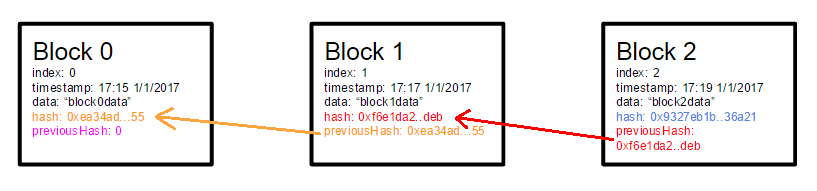
\includegraphics[width=0.7\textwidth]{blockchain_struttura.png}
  \caption{Sequnza di blocchi}
  \label{fig:blockchain_struttura}
\end{figure}

In questa sequenza di blocchi, ogni documento digitale è modificato dai client in diversi istanti di tempo e la catena mantiene un elenco di valori di timestamp relativi agli eventi accaduti sequenzialmente. I valori di timestamp non sono modificabili e in caso di controversie ogni modifica apportata al documento può essere consultata.

\subsection{Alberi di Merkle}
Dave Bayer, contribuì ad integrare la struttura per la marcatura temporale di Haber e Stornetta, con la realizzazione dei Merkle Tree (Alberi di Merkle) \cite{bayer1993improving}, offrendo l'opportunità di raccogliere più documenti in un singolo blocco (Figura \ref{fig:merkle_tree}). Tali alberi ricevono il nome da Ralph Merkle e in essi i nodi foglia sono contrassegnati da un blocco dati, mentre i nodi non-foglia dall'hash crittografico delle etichette dei loro nodi figlio. Detti anche Alberi di hash, mostrano una versione più generica di liste e catene hash e consentono una verifica sicura ed efficace del contenuto di grandi strutture dati.

\begin{figure}[h]
  \centering
  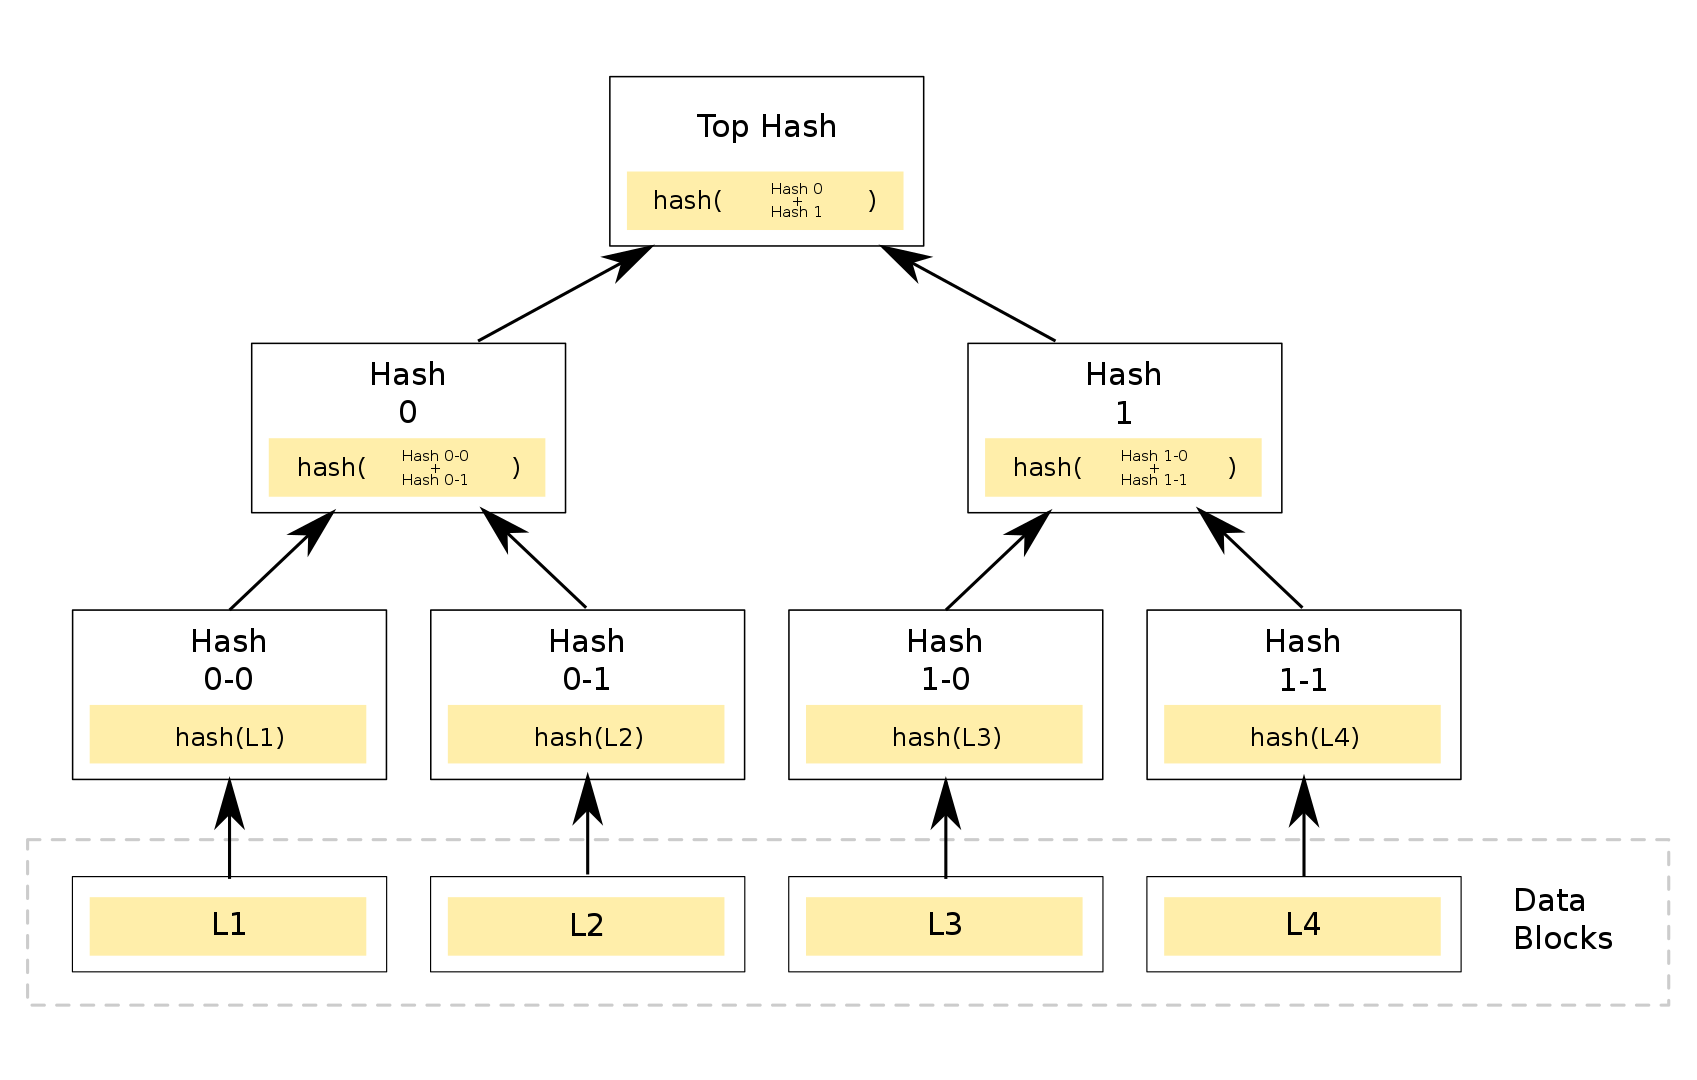
\includegraphics[width=0.7\textwidth]{merkle_tree.png}
  \caption{Esempio di albero di Merkle}
  \label{fig:merkle_tree}
\end{figure}

Nella figura \ref{fig:merkle_tree} possiamo vedere come i valori hash dei blocchi sono definiti "foglie", mentre i valori hash dei loro figli sono detti "nodi". Gli alberi di Merkle vengono utilizzati per rilevare incongruenze tra le repliche e per ridurre al minimo la quantità di dati.

\subsection{Bit gold}
Nel 2005, si ha avuto il primo tentativo di moneta decentralizzata grazie all'informatico Nick Szabo, il quale ha proposto una nuova valuta basata sulla blockchain: \textbf{Bit gold} \cite{szabo_2005}. Moneta che però non ha riscosso molto successo, ma nonostante ciò il 2005 rappresenta un anno cruciale nel contesto blockchain.

La proposta dell'informatico si basa sul calcolo di una stringa di bit a partire da una stringa di bit di sfida, utilizzando funzioni chiamate in vario modo "client puzzle function", "proof of work function" o "secure benchmark function". La stringa di bit risultante è la proof of work.

Ecco le fasi principali del sistema bit gold che Szabo ha definito:

\begin{enumerate}
  \item Viene creata una stringa pubblica di bit, la "stringa di sfida" (vedi passo 5).
  \item Alice sul suo computer genera la stringa di proof of work dai bit di sfida utilizzando una funzione di benchmark.
  \item La proof of work viene registrata in modo sicuro con un timestamp. Questo dovrebbe funzionare in modo distribuito, con diversi servizi di timestamp in modo che non sia necessario affidarsi a un particolare servizio di timestamp.
  \item Alice aggiunge la stringa di sfida e la stringa di proof of work con timestamp a un registro di proprietà distribuito per il bit gold. Anche in questo caso, non si fa affidamento su un singolo server per il corretto funzionamento del registro.
  \item L'ultima stringa creata di bit gold fornisce i bit di sfida per la stringa creata successivamente.
  \item Per verificare che Alice sia la proprietaria di una particolare stringa di bit gold, Bob controlla la catena di titoli non falsificabile nel registro dei titoli di bit gold.
  \item Per verificare il valore di una stringa di bit gold, Bob controlla e verifica i bit di sfida, la stringa di proof of work e il timestamp.
\end{enumerate}

Si noti che il controllo di Alice sul suo bit gold non dipende dal suo solo possesso dei bit, ma piuttosto dalla sua posizione di leader nella catena di titoli non falsificabile (catena di firme digitali) nel registro dei titoli.

Tutto questo può essere automatizzato da un software. I limiti principali alla sicurezza dello schema sono la capacità di distribuire la fiducia nelle fasi (3) e (4) e il problema dell'architettura della macchina, che verrà discusso di seguito.

Hal Finney ha implementato una variante di bit gold chiamata \textbf{RPOW (Reusable Proofs of Work)}. Si basa sulla pubblicazione del codice informatico della "zecca", che viene eseguito su un computer remoto a prova di manomissione. L'acquirente di bit gold può quindi utilizzare l'attestazione remota, che Finney chiama tecnica del server trasparente, per verificare che un determinato numero di cicli sia stato effettivamente eseguito.

Il problema principale di tutti questi schemi è che gli schemi di proof of work dipendono dall'architettura del computer, non solo da una matematica astratta basata su un "ciclo di calcolo" astratto. (Pertanto, potrebbe essere possibile essere un produttore a bassissimo costo (di diversi ordini di grandezza) e inondare il mercato di bit gold. Tuttavia, dal momento che il bit gold è marcato a tempo, il tempo creato e la difficoltà matematica del lavoro possono essere dimostrati automaticamente. Da ciò si può solitamente dedurre il costo di produzione in quel periodo.

A differenza degli atomi d'oro fungibili, ma come nel caso degli oggetti da collezione, una grande disponibilità in un determinato periodo di tempo farà scendere il valore di questi particolari oggetti. Da questo punto di vista, il "bit gold" si comporta più come gli oggetti da collezione che come l'oro. Tuttavia, la corrispondenza tra questo mercato ex post e l'asta che determina il valore iniziale potrebbe creare un profitto molto consistente per il "minatore di bit gold" che inventa e distribuisce un'architettura informatica ottimizzata.

Pertanto, il bit gold non sarà fungibile in base a una semplice funzione, ad esempio, della lunghezza della stringa. Per creare unità fungibili, i commercianti dovranno invece combinare unità di valore diverso.

\subsection{Bitcoin}
Bitcoin nasce ufficialmente agli inizi del 2009 con la creazione del "blocco genesi", ma se ne inizia a parlare nel 2008 a seguito della pubblicazione di un paper scientifico intitolato \textit{"Bitcoin: A Peer-to-Peer Electronic Cash System"} \cite{bitcoin-white-paper}.

\begin{figure}[h]
  \centering
  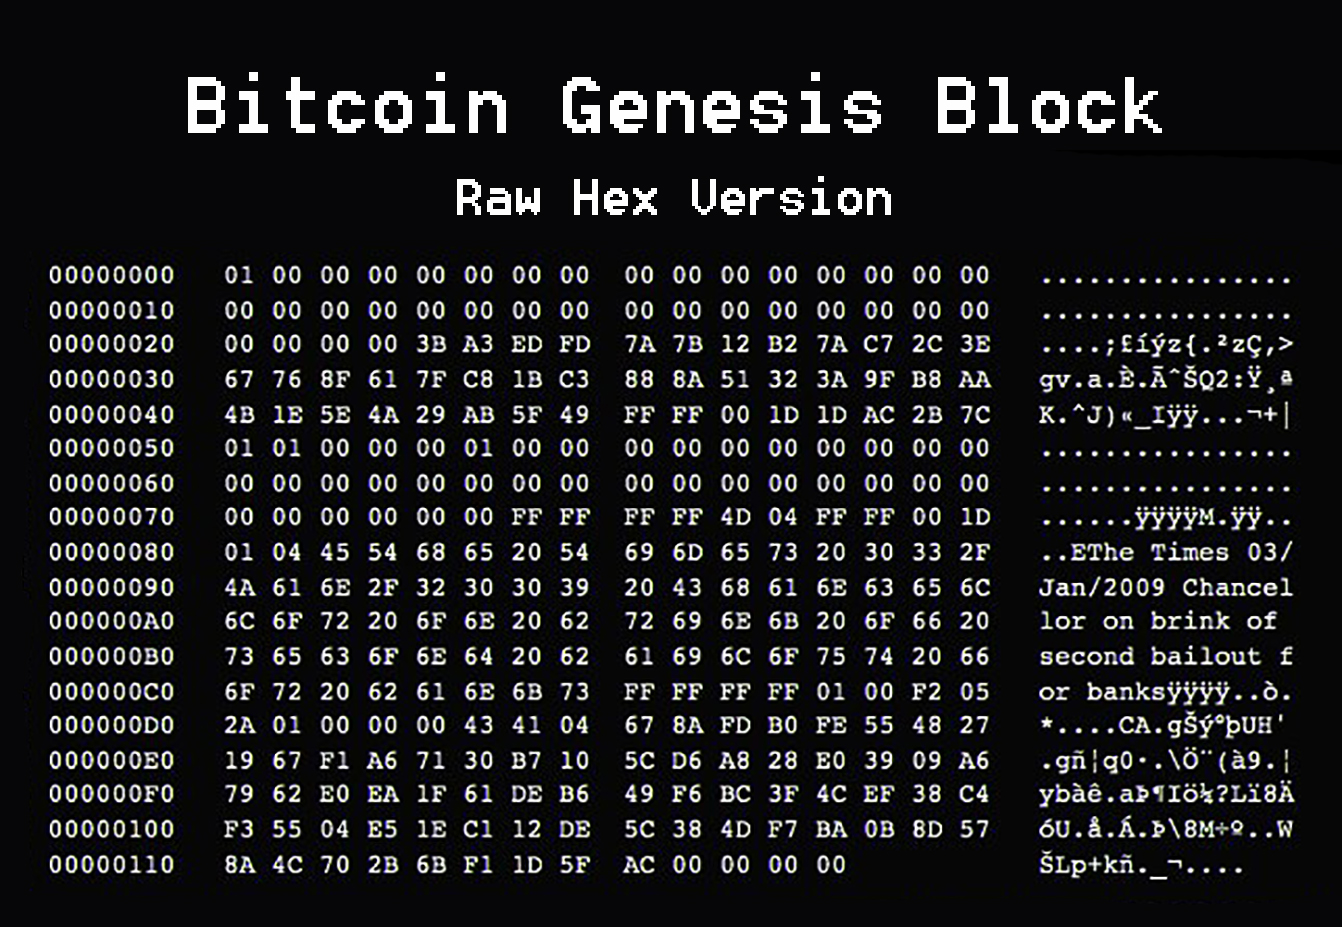
\includegraphics[width=0.7\textwidth]{bitcoin_genesis_block.jpeg}
  \caption{Messaggio di Satoshi Nakamoto incorporato nella coinbase del primo blocco}
  \label{fig:bitcoin_genesis_block}
\end{figure}

Il \textbf{libro bianco o "whitepaper" di Bitcoin} fu pubblicato in un articolo scientifico tramite Cryptography Mailing List nel mese di \textbf{ottobre del 2018}. Essendo pubblicato in modo anonimo sotto lo pseudonimo Satoshi Nakamoto genera ancora più mistero e confusione. Così tanto che ancora oggi si cerca un vero nome dietro quel soprannome.

\textit{Prima di iniziare è bene fare una precisazione: bitcoin con la b minuscola è la moneta digitale, Bitcoin con la b maiuscola è il protocollo che la governa.}

L'obiettivo di Satoshi era quello di creare un sistema di pagamento tramite una versione puramente peer-to-peer di denaro elettronico che permetterebbe di effettuare pagamenti online da un'entità ad un'altra senza passare tramite un'istituzione finanziaria centrale. I nodi peer-to-peer, che costituiscono la rete, non formano gerarchie client-server ma agiscono al contempo sia da client che da server.

Le firme digitali offrono una soluzione parziale al problema, ma i benefici principali sono persi se una terza persona di fiducia è ancora richiesta per prevenire la doppia spesa. Ovvero, quando un utente fa una transazione ci deve essere la garanzia che i soldi appena spesi non possano essere utilizzati una seconda volta per compierne un'altra, problema illustrato in Figura \ref{fig:double_spending}.

La moneta fisica risolve alla radice questo problema non potendo esistere in due luoghi contemporaneamente. In merito ai pagamenti digitali, in un sistema di fiducia centralizzato il problema è gestito da una terza parte che fa controlli su ogni operazione effettuata dagli utenti.

\begin{figure}[htbp]
  \centering
  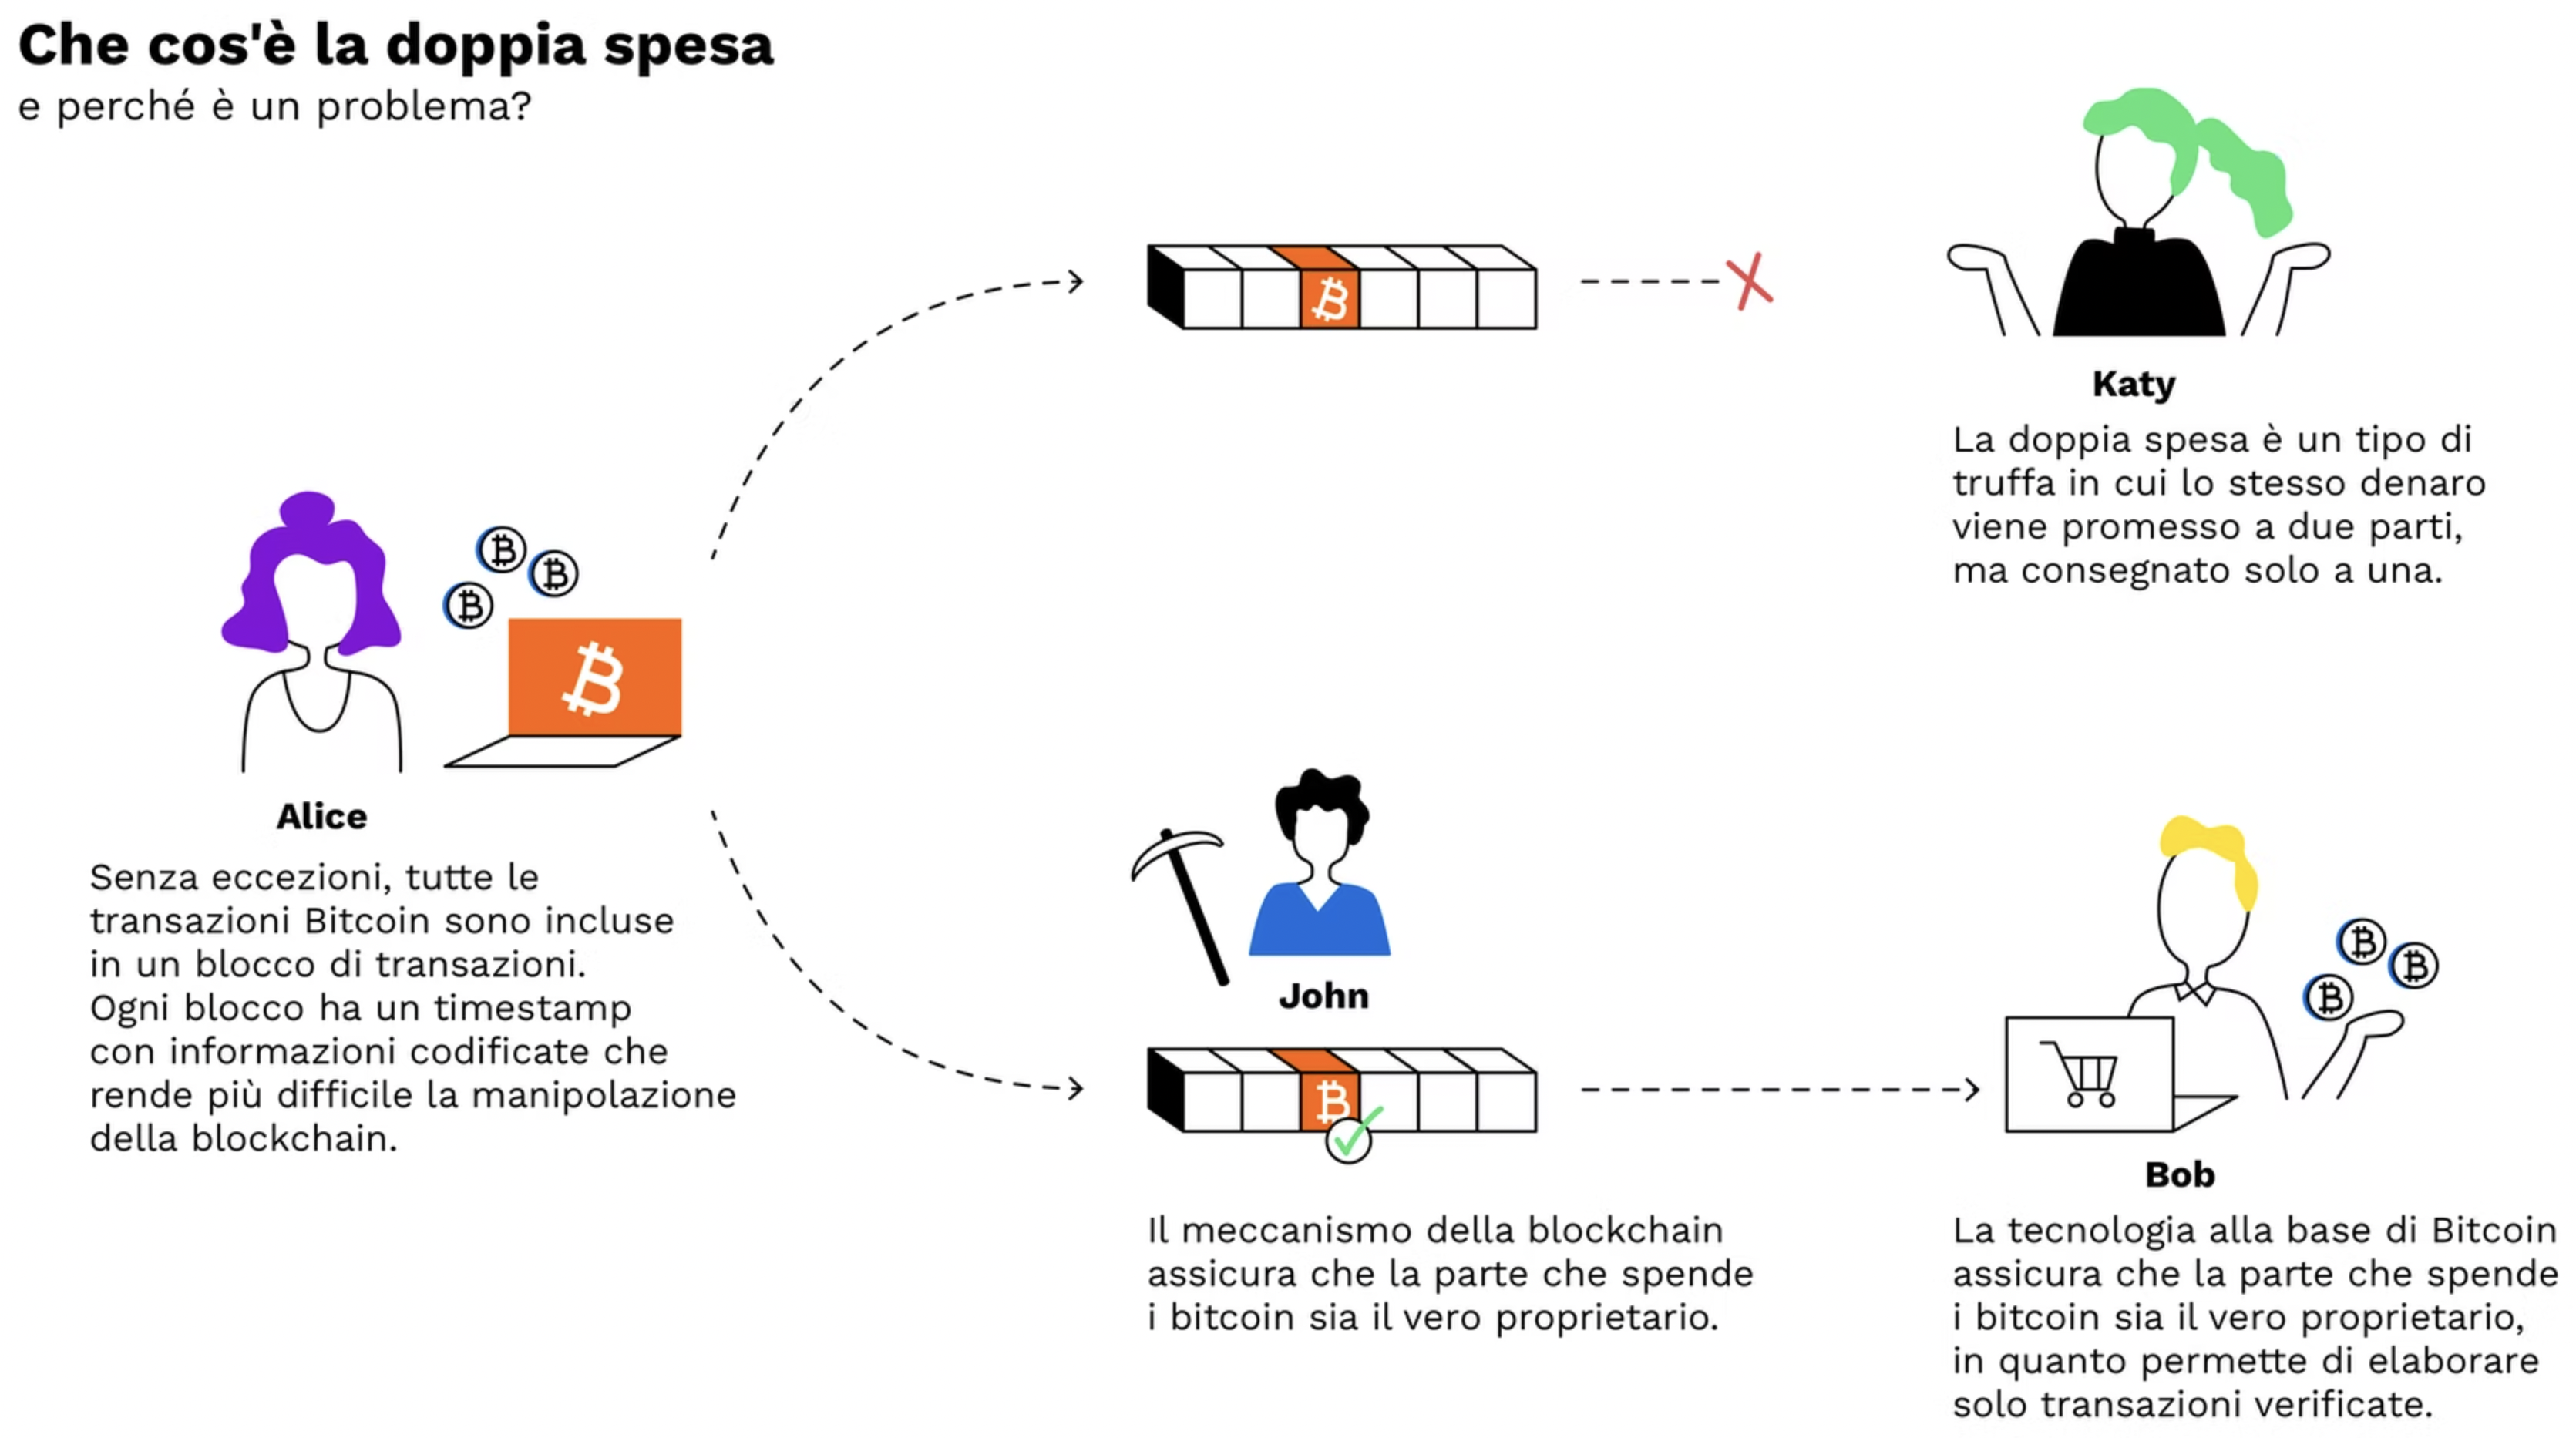
\includegraphics[width=0.7\textwidth]{double_spending.png}
  \caption{Problema del double spending}
  \label{fig:double_spending}
\end{figure}

Satoshi propone una soluzione al problema della doppia spesa mediante l'utilizzo di una rete peer-to-peer, includendo elementi di crittografia.

La legge di mercato della domanda e offerta determinano il valore economico assunto dal bitcoin. Bitcoin è quotato su siti appositi chiamati Exchange. Tali siti permettono di scambiare Bitcoin con Euro, Dollaro Americano o altre monete emesse dai governi, dette anche \textbf{monete fiat}\footnote{Moneta legale (o moneta a corso legale o, ancora, moneta fiduciaria)}. Il primo Exchange è andato online nel marzo del 2010 e quotava bitcoin a soli 0,003\$. Il 22 maggio 2010 vengono acquistate due pizze in Florida per 10.000,00 bitcoin. Meno di un anno dopo la criptomoneta raggiunge il valore di 1,00\$. Nel 2013 la valutazione subisce alti e bassi arrivando a toccare un massimo di 1200,00\$. Con l'apertura di nuovi exchange e grazie alla speculazioni da parte di un numero sempre maggiore di utenti il prezzo sale fino a 10.000,00\$ a novembre 2017. Oggi (fine luglio 2022) ha un valore di 20.893,00\$ circa. L'andamento del bitcoin è illustrato in Figura \ref{fig:bitcoin_quotation}.

\begin{figure}[htbp]
  \centering
  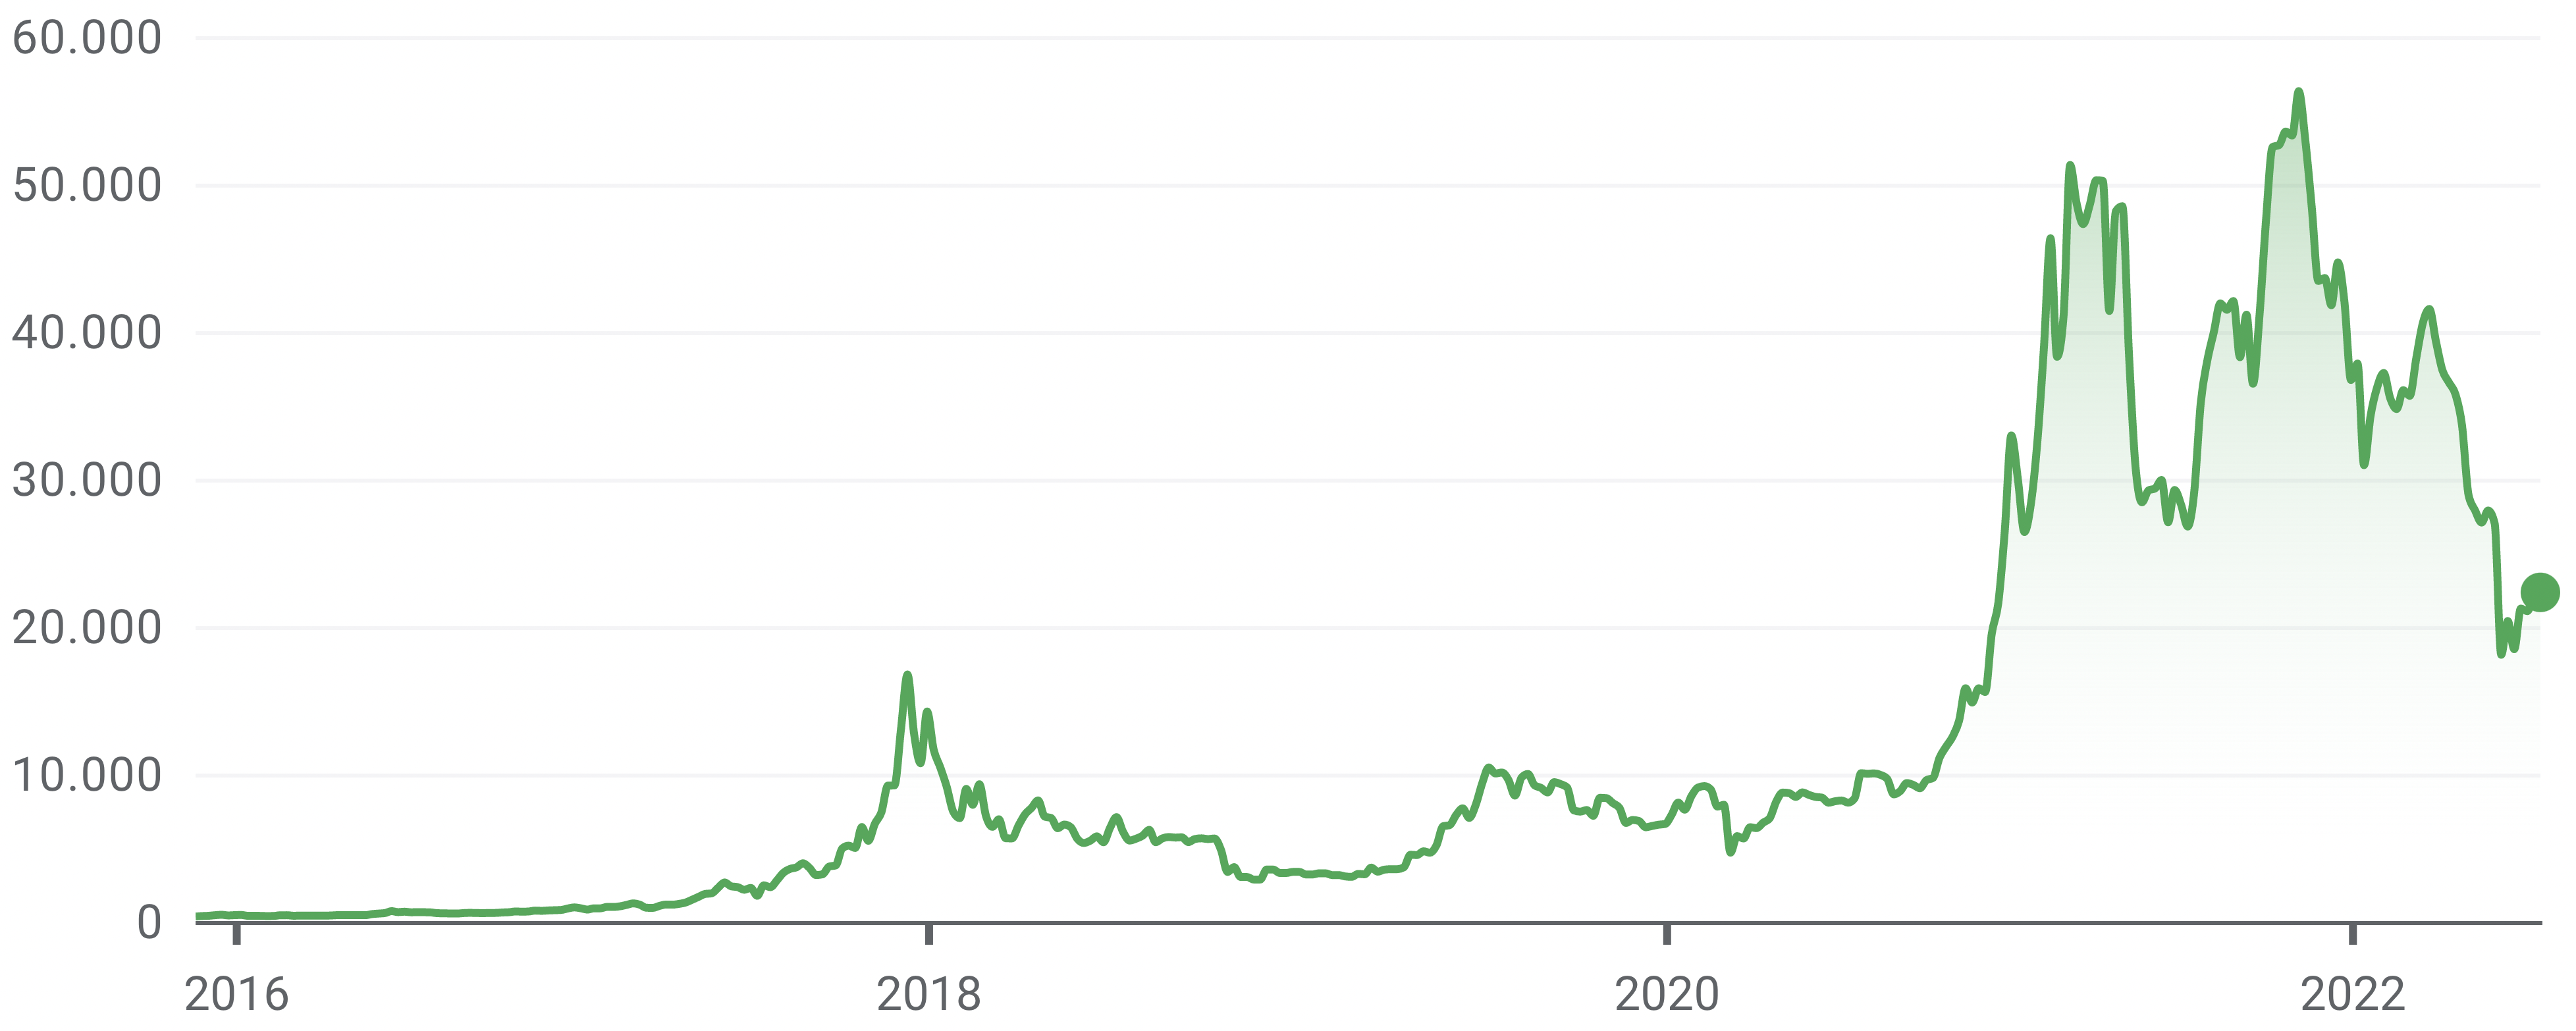
\includegraphics[width=0.7\textwidth]{bitcoin_quotation.png}
  \caption{Andamento del bitcoin}
  \label{fig:bitcoin_quotation}
\end{figure}

\section{Cos'è la blockchain}
La blockchain è una sottofamiglia di tecnologie in cui il registro è strutturato come una catena di blocchi contenenti le transazioni e la cui validazione è affidata a un meccanismo di consenso, distribuito su tutti i nodi della rete nel caso delle \textit{blockchain permissionless o pubbliche} o su tutti i nodi i nodi che sono autorizzati a partecipare al processo di validazione delle transazioni da includere nel registro nel caso delle \textit{blockchain permissioned o private}.

Per alcuni, la blockchain è la nuova generazione di Internet, o meglio ancora è la Nuova Internet. Si ritiene che possa rappresentare una sorta di Internet delle Transazioni arrivndo a creare e rappresentare la Internet del Valore sulla base di sette caratteristiche \cite{bellini_2021}:

\begin{enumerate}
  \item \textbf{Decentralizzazione}
  \item \textbf{Trasparenza}
  \item \textbf{Sicurezza}
  \item \textbf{Immutabilità}
  \item \textbf{Consenso}
  \item \textbf{Responsabilità}
  \item \textbf{Programmabilità}
\end{enumerate}

Partendo da questi principi, la blockchain introduce un nuovo concetto di fiducia al punto che alcuni ritengono che la blockchain possa assumere anche un valore per certi aspetti di tipo “sociale e politico": le operazioni avvengono in modo onesto e trasparente, senza la dipendenza da un supervisore.

Bisogna però distinguere la blockchain dalla Blockchain Bitcoin, che è la prima Blockchain. A questa identificazione si è sovrapposta anche quella con la criptocurrency bitcoin e ha portato un pò a "confondere" la blockchain con altri ambiti di innovazione come le digital currency. Forse per quest'ultima ragione la blockchain è stata spesso associata ad un concetto di digital currency alternativa o complementare e di digital payment. In realtà, come vedremo, la blockchain è un fenomeno assai più ampio e articolato.

\subsection{Architettura della blockchain}
La tecnologia blockchain è un database pubblico decentralizzato che tiene testimonianza di chi possiede beni digitali e di chi effettua transazioni attraverso una rete peer-to-peer. Queste sono protette da crittografia e raccolte cronologicamente all'interno di blocchi di dati, a loro volta protetti e collegati. In tal modo viene creato un registro immutabile, che tiene traccia di tutte le transazioni effettuate, replicato su ogni computer che sfrutta la rete. La blockchain può essere considerata come un insieme di meccanismi interconnessi che forniscono funzionalità specifiche all'infrastruttura, come illustrato in Figura \ref{fig:blockchain_architettura}.

\begin{figure}[htbp]
  \centering
  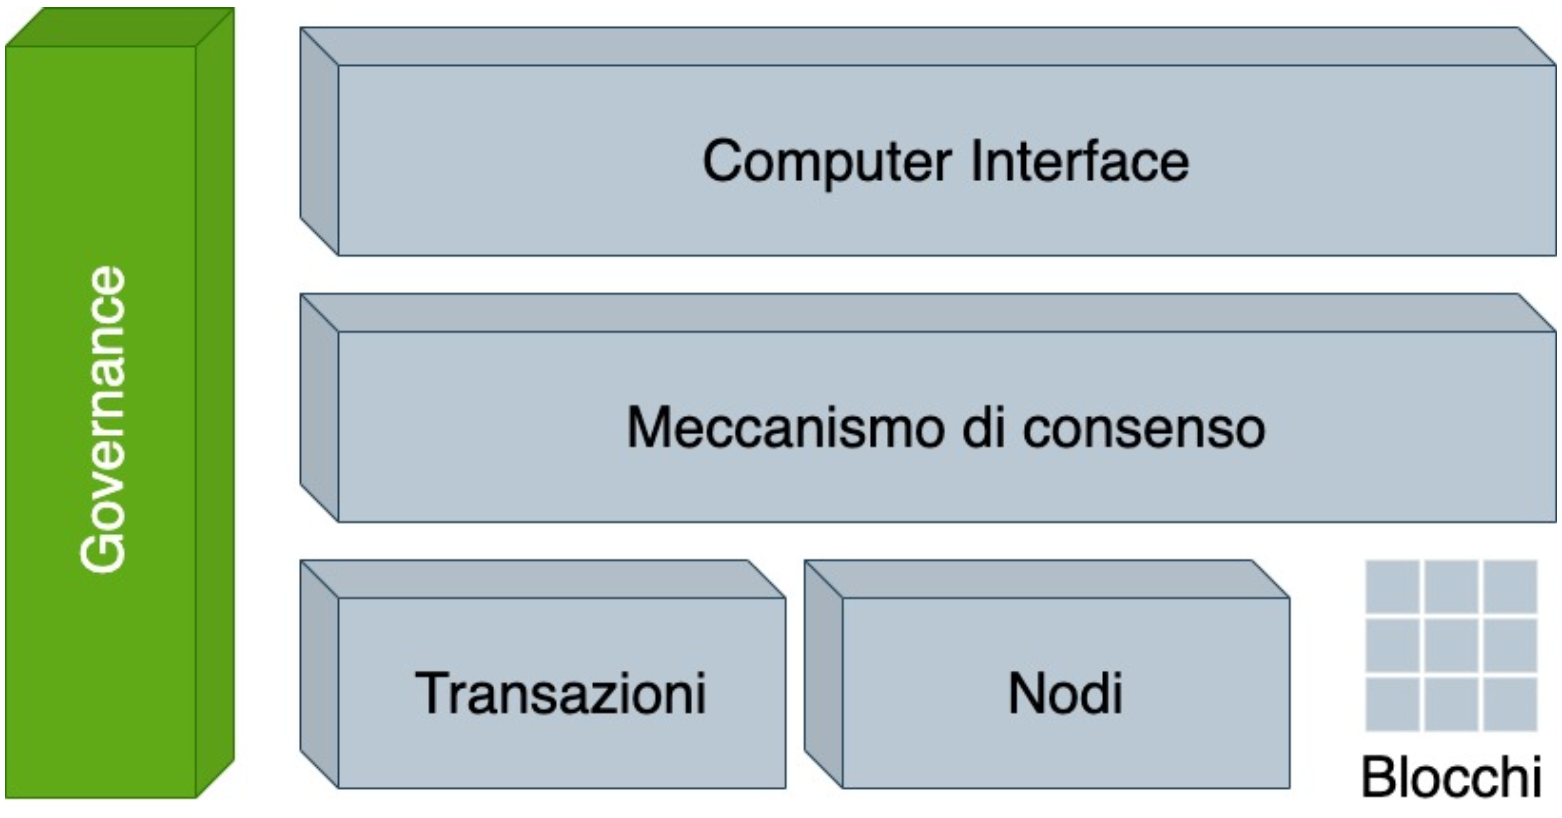
\includegraphics[width=0.7\textwidth]{blockchain_architettura.png}
  \caption{Architettura della blockchain di bitcoin}
  \label{fig:blockchain_architettura}
\end{figure}

Alla base di questa infrastruttura ci sono le \textbf{transazioni}, firmate tra i peers. Queste indicano un accordo tra due partecipanti, che può comportare il trasferimento di risorse fisiche o digitali. Almeno un partecipante firma questa transazione, poi divulgata ai suoi vicini. L'entità connessa alla blockchain è chiamata \textbf{nodo} e i nodi che verificano tutte le regole blockchain sono chiamati nodi completi (\textbf{miner}). Questi raggruppano le transazioni in \textbf{blocchi} e determinano se le transazioni sono valide, quindi conservate nella blockchain, e quali no.

Al livello del \textbf{Meccanismo di consenso}, i nodi devono raggiungere un accordo su quali transazioni devono essere mantenute nella blockchain per garantire che non ci siano rami corrotti e divergenze.
La \textbf{Computer Interface} permette alle blockchain di offrire più funzionalità: mentre una blockchain memorizza uno stato, ad esempio l'insieme di tutte le transazioni effettuate dagli utenti, la Computer Interface permette di memorizzare stati complessi che vengono aggiornati dinamicamente utilizzando il calcolo distribuito.
Infine, il livello di \textbf{Governance} estende l'architettura blockchain coprendo le interazioni umane che avvengono nel mondo fisico. I protocolli blockchain sono influenzati da input di diversi gruppi di persone che integrano nuovi metodi, migliorano i protocolli e applicano patch al sistema. Benchè queste parti siano necessarie per la crescita di ciascuna blockchain, costituiscono processi esterni alla catena. Per cui, la governance della blockchain si occupa di come questi diversi attori si uniscono per produrre, mantenere o modificare gli input che compongono una blockchain.

\subsection{Funzionamento della Blockchain}
Prendendo in considerazione la più famosa blockchain e cioè la blockchain di Bitcoin, verranno di seguito analizzate le caratteristiche ed il funzionamento generale della tecnologia blockchain. I suoi principali elementi sono:

\begin{itemize}
  \item Nodi
  \item Transazioni
  \item Hash
  \item Blocchi
  \item Registro (Ledger)
  \item Nodi completi (Miner)
\end{itemize}

\subsubsection{Hashing}
Viene utilizzata una funzione hash \(h\), per convertire un messaggio di una certa lunghezza in una stringa di dimensioni fisse che genera valori hash (digest). La mappatura avviene in maniera tale da non consentire di risalire al messaggio originale partendo dalla stringa, la cui lunghezza è direttamente proporzionale al livello di sicurezza della funzione. Una funzione hash ideale dovrebbe:

\begin{enumerate}
  \item Conteggiare facilmente i valori hash, per qualsiasi dato a disposizione;
  \item Generare i medesimi digest per due o più input uguali;
  \item Garantire difficoltà di previsione dei digest conoscendo i dati in ingresso;
  \item Ostacolare di risalire alle informazioni iniziali a prescindere dalla tipologia di input;
  \item Generare valori hash molto diversi tra loro anche per input simili.
\end{enumerate}

A seconda dell'algoritmo adottato varia la lunghezza dei digest. Bitcoin
usa l'algoritmo \textbf{SHA-256} che restituisce un output di 256 bit.

Ecco un esempio:
\begin{quote}
  \$ hash("Ciao, Mondo!");

  \textit{SDFSDF98S8J9238FJ130F2K3FM23F0MI23923F023F230MF203F}
\end{quote}

\subsubsection{Nodi, transazioni e blocchi}
La \textbf{transazione} è un'operazione di scambio di risorse fisiche o digitali tra utenti (\textbf{nodi}) connessi ad una rete peer-to-peer. Al suo interno saranno contenuti gli indirizzi pubblici dei nodi coinvolti nello scambio, l'amount della transazione e la firma digitale del mittente (Figura \ref{fig:sitir}).

\begin{figure}[htbp]
  \centering
  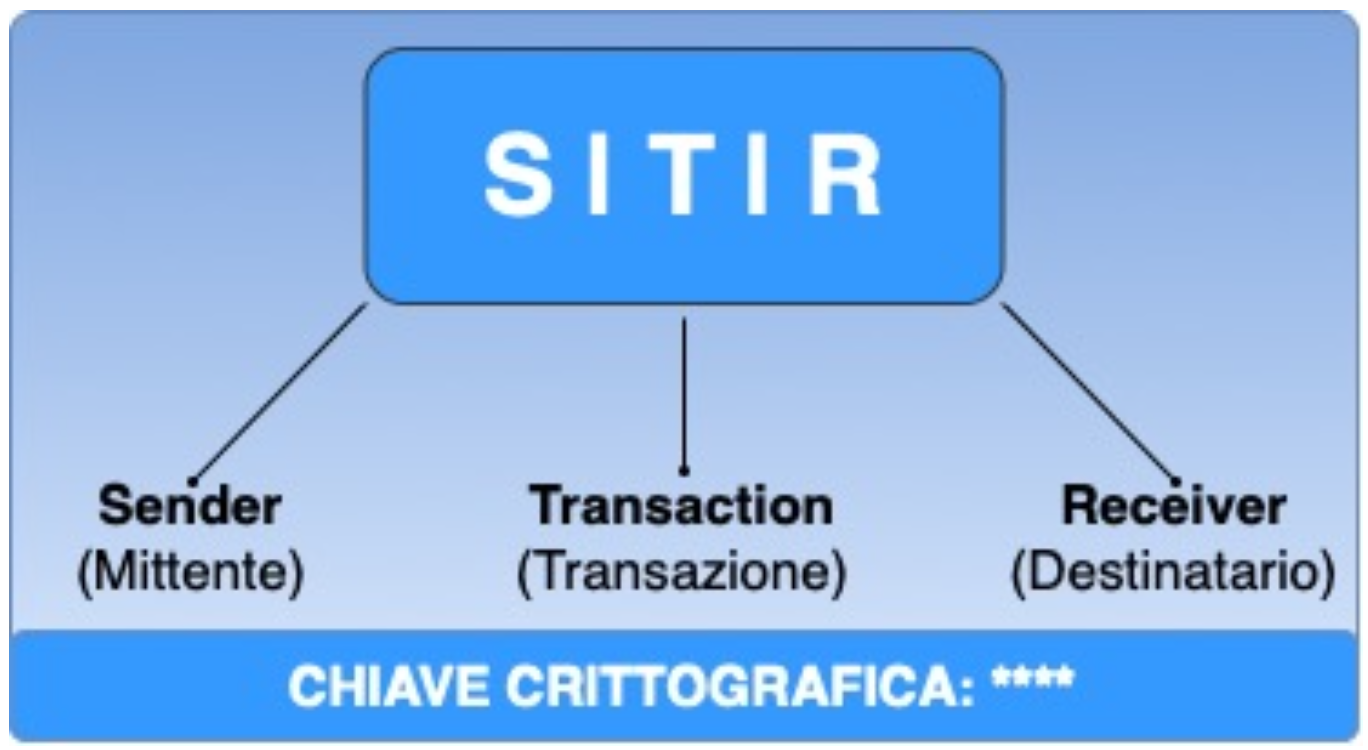
\includegraphics[width=0.7\textwidth]{sitir.png}
  \caption{Principali componenti della transazione}
  \label{fig:sitir}
\end{figure}

Le firme digitali sono utili ai nodi per dimostrare la loro identità senza rivelare la propria chiave privata. La firma è il risultato della combinazione tra la chiave privata del mittente e la funzione hash (Figura \ref{fig:hash_in_transazione}).

\begin{figure}[htbp]
  \centering
  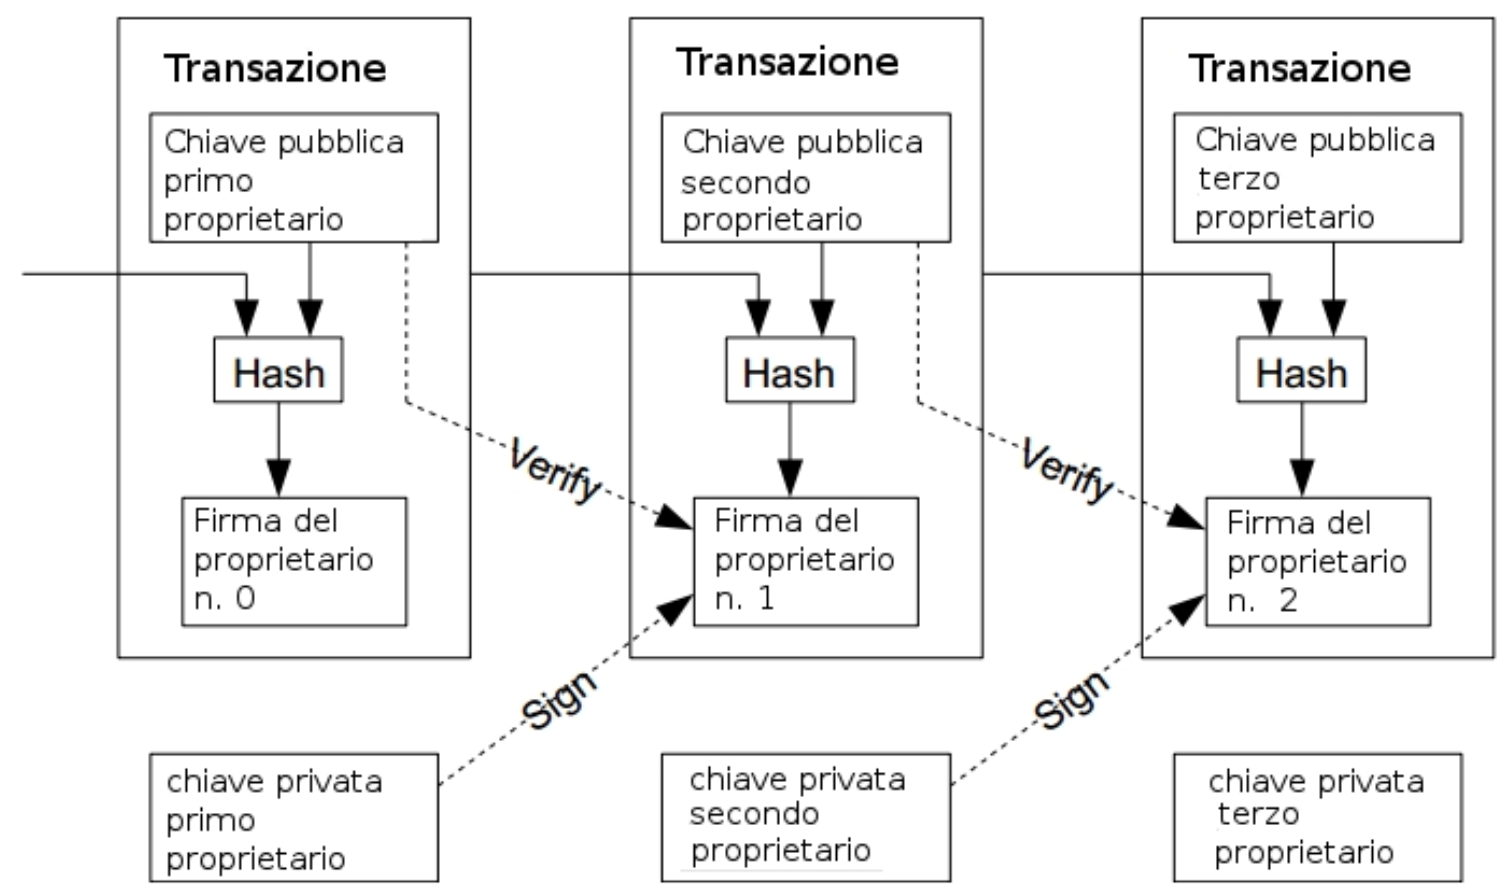
\includegraphics[width=0.7\textwidth]{hash_in_transazione.png}
  \caption{Uso della firma digitale nelle transazioni}
  \label{fig:hash_in_transazione}
\end{figure}

Il destinatario riceve i dati crittografati insieme alla firma digitale, e sfruttando la chiave privata del mittente, può decifrare i dati. La chiave pubblica è stata precedentemente condivisa tra gli utenti coinvolti o consultabile all'interno del server. L'algoritmo usato per la creazione della firma digitale è l'\textit{Elliptic Curve Digital Signature Algorithm (ECDSA)}[19].
I \textbf{blocchi}, unità fondamentali della catena, sono caratterizzati da un insieme di transazioni, un timestamp che li colloca temporalmente, un valore hash posto nell'header (Figura \ref{fig:multi_sitir}) e l'hash dei blocchi precedenti, in modo tale da poter monitorare lo stato attuale della catena anche a seguito dell'aggiunta di nuovi blocchi. Come possiamo vedere nella (Figura \ref{fig:hash_chain}), ogni blocco contiene più transazioni, un valore hash proprio e quello del blocco precedente: forma una catena di hash o blockchain. L'ordine dei blocchi è deterministico. Ogni nodo conserva una copia dell'intera blockchain, in modo da poter verificare ogni transazione.

\begin{figure}[htbp]
  \centering
  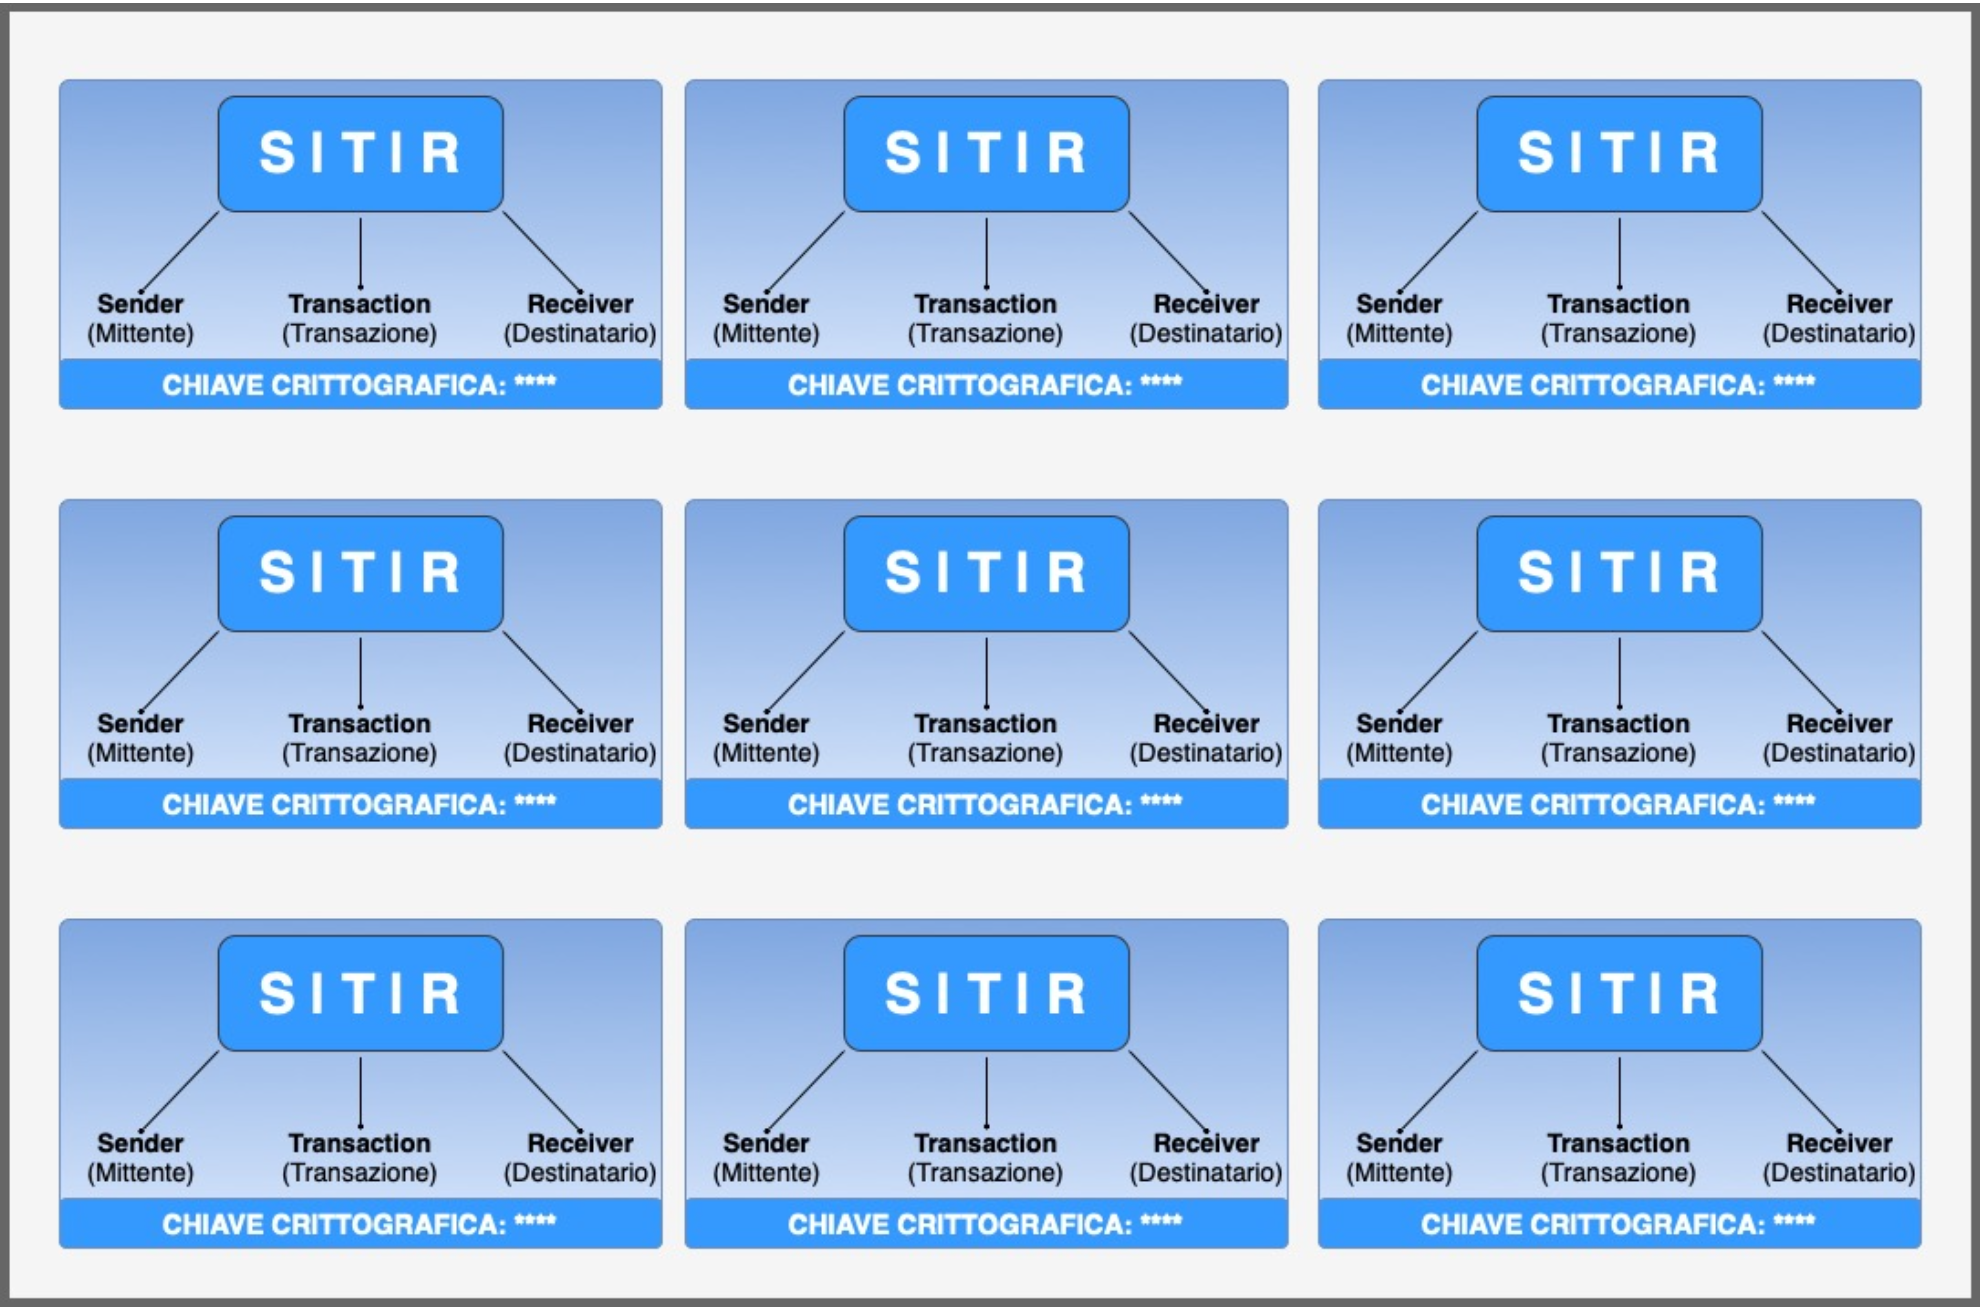
\includegraphics[width=0.7\textwidth]{multi_sitir.png}
  \caption{Struttura di un blocco contenente diverse transazioni}
  \label{fig:multi_sitir}
\end{figure}

\begin{figure}[htbp]
  \centering
  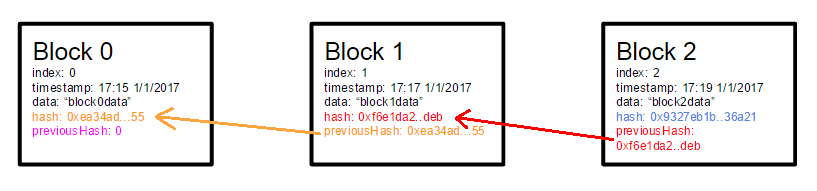
\includegraphics[width=0.7\textwidth]{blockchain_struttura.png}
  \caption{Hash Chain}
  \label{fig:hash_chain}
\end{figure}

\subsubsection{Il registro (Ledger)}
Abbiamo tre tipi di network differenti:
\begin{description}
  \item[Rete centralizzata (Centralized Network)] I dati vengono raccolti all'interno di un'unica macchina, alla quale gli utenti si connettono per accedere alle informazioni desiderate. Si crea un \textit{single-point-of-failure}. Se l'intermediario centrale non è attivo o viene attaccato, l'intera rete smette di funzionare (Figura \ref{fig:tipologie_reti} Sinistra).
  \item[Rete Decentralizzata (Decentralized Network)] Non esiste un'unica macchina per l'archiviazione dei dati in quanto più server lavorano assieme per fornire agli utenti le informazioni desiderate. Non contiene \textit{single-point-of-failure}. Se uno dei nodi, è inattivo o è attaccato, il resto della rete può ancora funzionare normalmente (Figura \ref{fig:tipologie_reti} Centro).
  \item[Rete Distribuita (Distributed Network)] Non esiste alcuna macchina specializzata all'archiviazione dei dati, in quanto ogni singolo nodo della rete contiene le medesime informazioni. Tutti i nodi possono vedere tutto ed esiste un meccanismo di timestamp distribuito (Figura \ref{fig:tipologie_reti} Destra).
\end{description}

\begin{figure}[htbp]
  \centering
  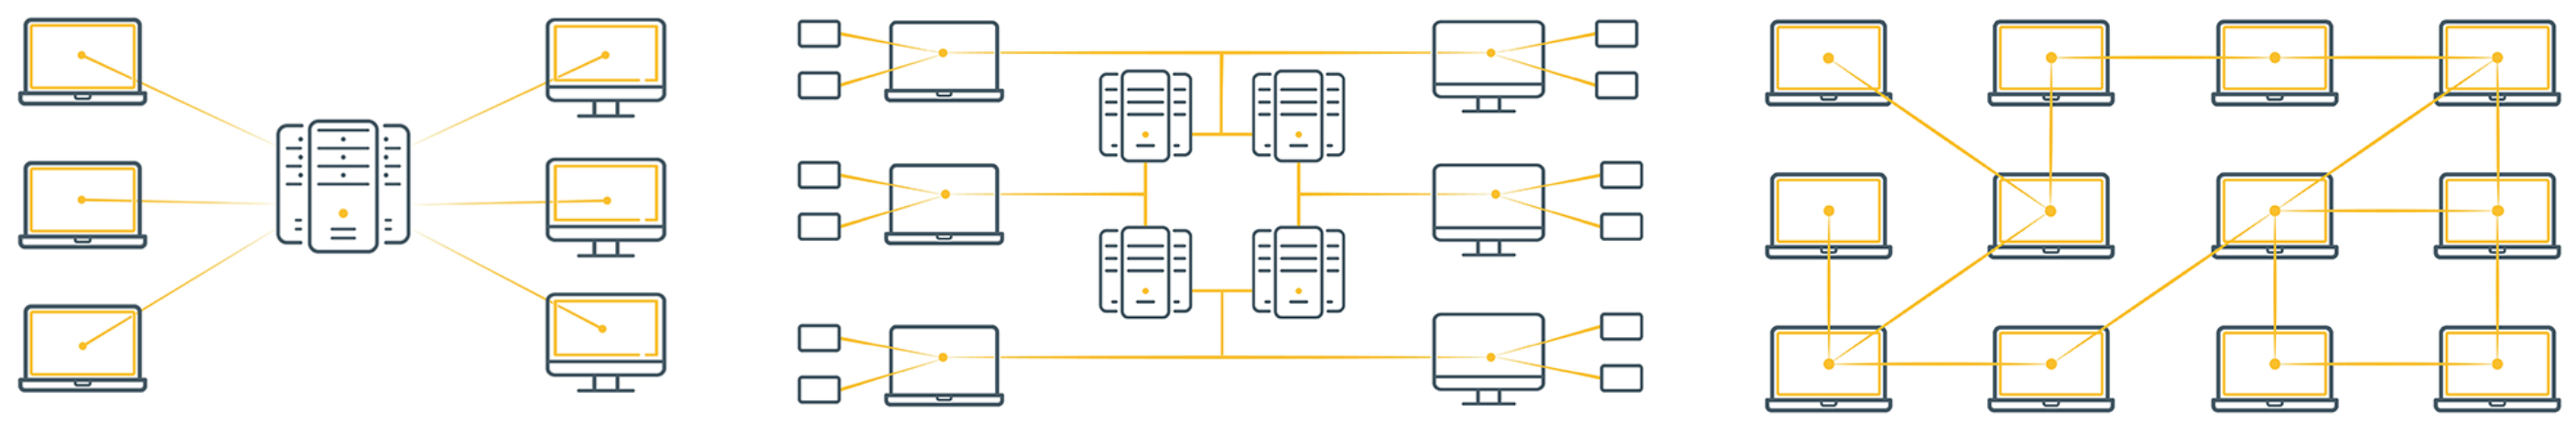
\includegraphics[width=1\textwidth]{tipologia_reti.png}
  \caption{Confronto delle tipologie di rete}
  \label{fig:tipologie_reti}
\end{figure}

L'ultima configurazione è tipica della tecnologia blockchain nella quale il registro, definito anch'esso distribuito, tiene nota di tutte le transazioni avvenute all'interno della rete e offre informazioni aggiornate sullo stato attuale della catena. La configurazione distribuita è più sicura di quella centralizzata per due motivi: in primis non esiste un punto vulnerabile centrale; in secondo luogo la potenza di calcolo richiesta ad un hacker per modificare una transazione all'interno di un blocco, e di conseguenza in tutti i blocchi della catena, non è raggiungibile con le attuali tecnologie.

\section{Algoritmi di consenso}
\subsection{Proof of Work}
L'algoritmo di consenso adottato dalla Bitcoin blockchain è il protocollo \textit{Proof-of-Work (PoW)} illustrato in Figura \ref{fig:bitcoin_pow}.

\begin{figure}[htbp]
  \centering
  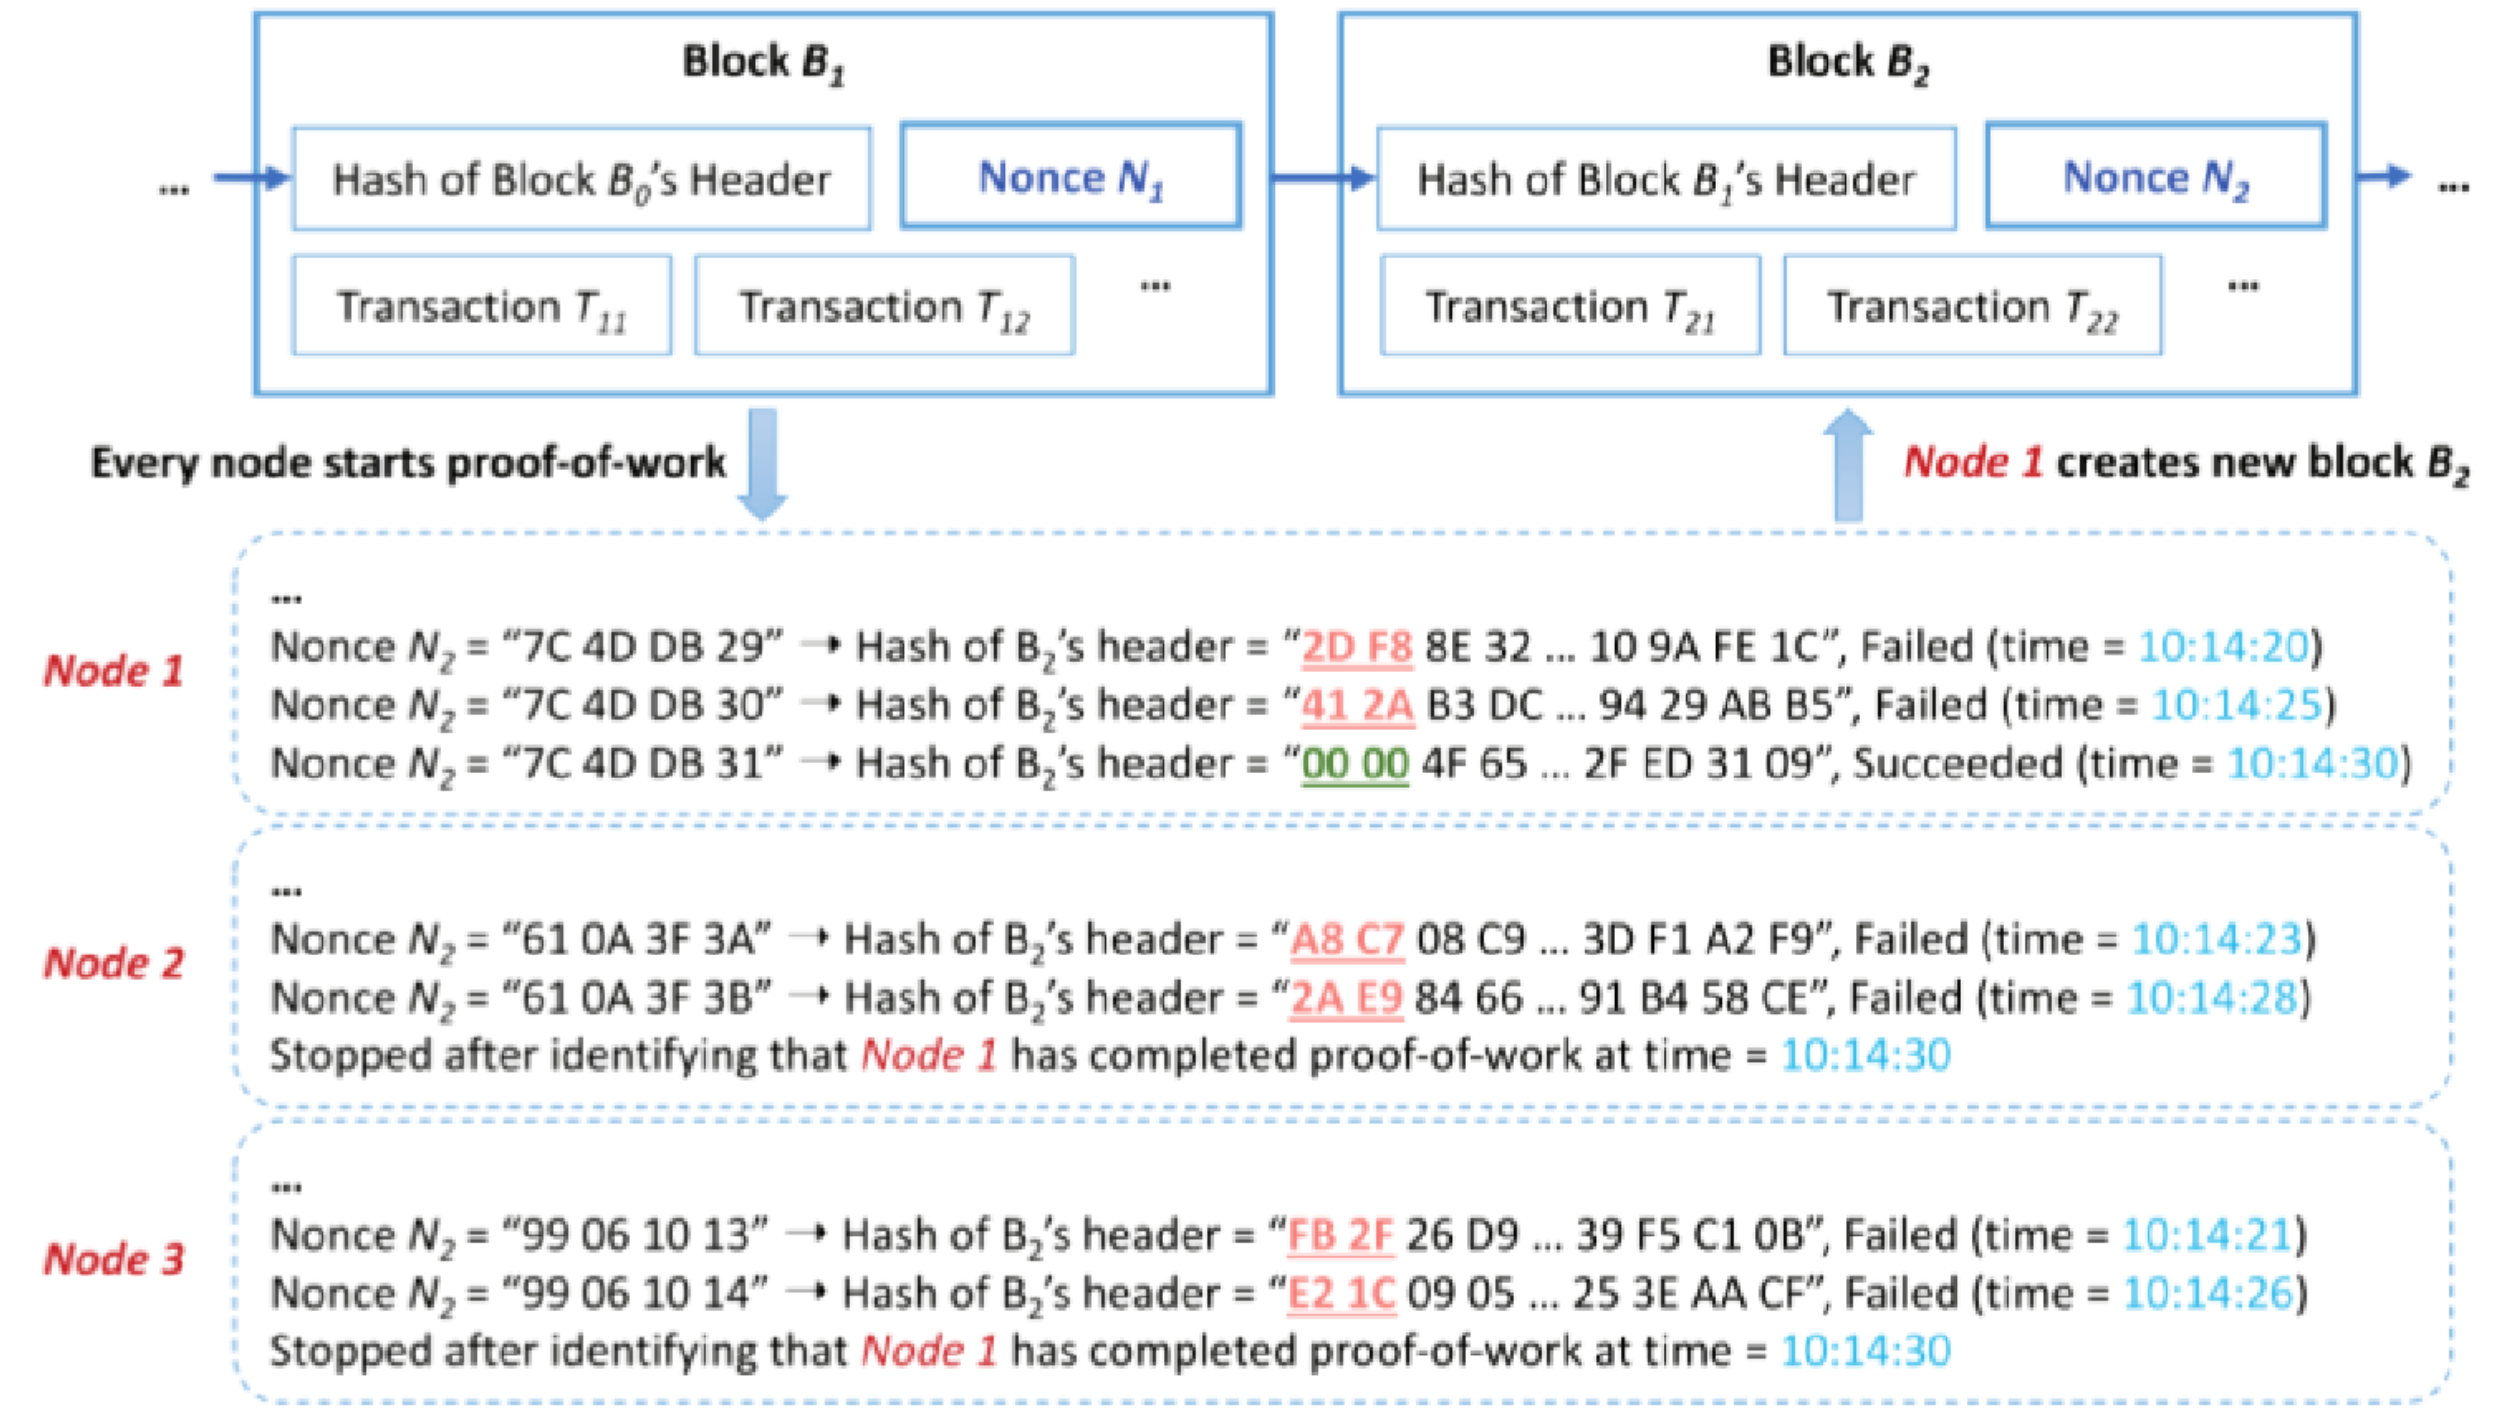
\includegraphics[width=1\textwidth]{bitcoin_pow.png}
  \caption{Meccanismo Proof-of-Work di bitcoin}
  \label{fig:bitcoin_pow}
\end{figure}

Per provare (\textbf{proof}) il lavoro di hashing, il \textit{nonce}\footnote{Generalmente di 32 bit, è un contatore aggiunto al blocco che funge da input della funzione hash} viene incrementato di 1 bit per ogni calcolo dell'hash (\textbf{work}) finchè il digest da 256 bit (SHA-256) non conterrà 16 bit zero iniziali (target).
Le transazioni non confermate vengono raccolte in un pool di memoria per ciascun nodo, mentre al primo nodo che riesce a completare la Proof-of-Work, viene concessa la creazione di un nuovo blocco, la verifica delle transazioni, lo spostamento delle transazioni confermate in un nuovo blocco al fine di allungare la catena e una ricompensa (token). Questo processo è detto mining nella blockchain Bitcoin, e i nodi coinvolti sono i miner. Essi sono chiamati ad affrontare dei problemi computazionali proposti dall'algoritmo, al fine di convalidare nuovi blocchi della catena a seguito della loro risoluzione. Tra i problemi troviamo:

\begin{itemize}
  \item Individuare un input partendo dal digest della funzione hash;
  \item Scomposizione in numeri primi;
  \item \textit{Guided tour puzzle control}: ad alcuni nodi è richiesto il calcolo di una funzione di hash in caso di attacco \textit{DoS (Denial of Service)}.
\end{itemize}

La difficoltà del problema è proporzionale al numero di miner, alla potenza di calcolo e al carico della rete e deve essere bilanciata: se troppo elevata rallenta la creazione dei blocchi, se troppo bassa rende la rete facilmente attaccabile. La creazione di un blocco richiede mediamente 10 minuti. Il problema in Bitcoin è definito Hashcash, e l'utente che riesce a risolverlo è ricompensato in Bitcoin Figura \ref{fig:hashcash}.

\begin{figure}[htbp]
  \centering
  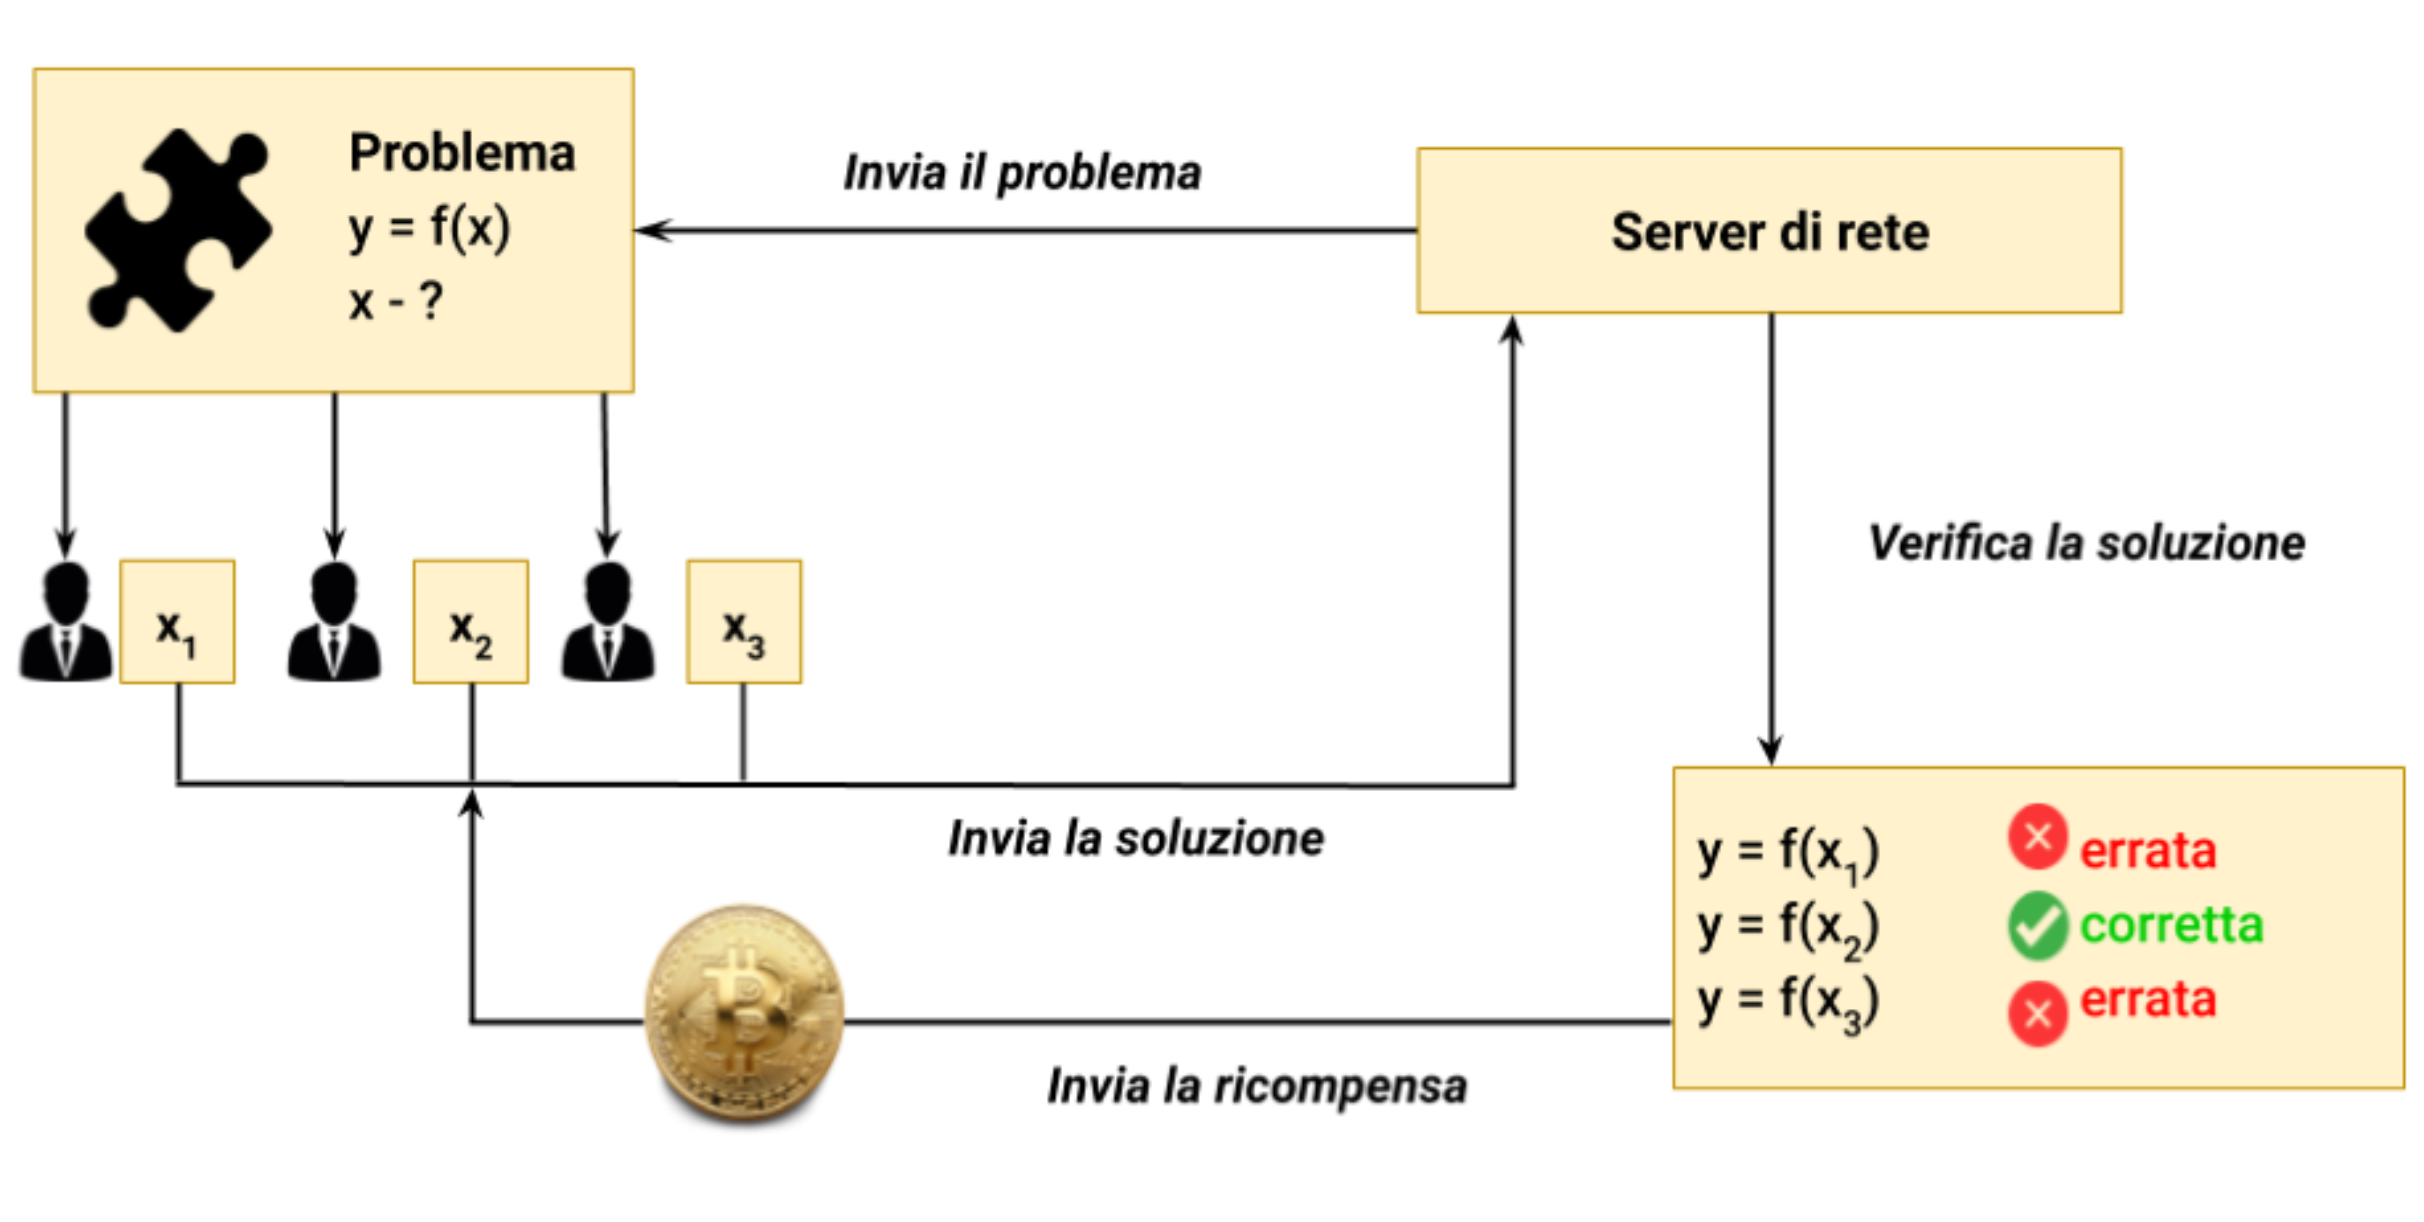
\includegraphics[width=0.7\textwidth]{hashcash.png}
  \caption{Esempio di funzionamento di Hashcash}
  \label{fig:hashcash}
\end{figure}

Sulla base di quanto visto fin qui, la tecnologia blockchain può definirsi \textbf{sicura}, \textbf{trasparente}, \textbf{immutabile} e \textbf{trustless}.

\subsection{Proof of Stake}
La \textit{Proof-of-Stake} è un metodo di verifica alternativo alla Proof-of-Work. Non viene difatti più usata l'idea di dover dimostrare di aver svolto dei calcoli fornendo un risultato computazionalmente complesso da calcolare, bensì viene introdotto un nuovo concetto, la \textit{coin age}. Essa serve per dimostrare di avere interesse nella gestione della moneta e acquisire quindi la fiducia della comunità per la fase di mining. La coin age è facile da calcolare: ad esempio se Bob ha ricevuto 10 coin da Alice e li ha posseduti per 90 giorni, Bob ha 900 coin-days di coin age. Quando Bob spenderà quei 10 coin ricevuti da Alice, la coin age accumulata da Bob con quei coin sarà detta consumata (o distrutta).

\subsubsection{Scelta del blocco successivo}
Ogni qualvolta un nuovo blocco è aggiunto alla blockchain, deve essere scelto il creatore del blocco successivo. Poichè quest'ultimo non può essere l'account che possiede la maggiore quantità della criptovaluta (altrimenti potrebbe creare tutti i blocchi), sono stati ideati diversi metodi di selezione:

\begin{description}
  \item[Selezione casuale] Nei BlackCoin è utilizzata una funzione casuale per predire il generatore del blocco successivo, impiegando una formula che cerca il valore hash più basso rapportato alla dimensione della somma in gioco. Essendo quest'ultimo pubblico, è facile fare previsioni su quale account si aggiudicherà il diritto di minare il nuovo blocco.
  \item[Selezione basata sulla velocità] Per evitare di far accumulare agli utenti grandi quantità di monete ed aumentare il proprio patrimonio di coin age, alcune monete come i Reddcoin scelgono il minatore successivo in base alla velocità di movimentazione, incoraggiando quindi lo scambio di moneta.
  \item[Selezione basata sul voto] A differenza di altre monete che si basano su funzioni del tutto estranee ad interventi umani diretti, alcune monete come i BitShares hanno implementato un sistema che permette agli utenti di votare e scegliere chi far diventare il minatore successivo.
  \item[Selezione basata sull'anzianità] Nei PPCoin è stato introdotto, affiancato ad una selezione casuale, il concetto di anzianità. L'anzianità è misurata in coin age, valore calcolato considerando solamente monete non spese per almeno 30 giorni e non più di 90, ciò permette di non avere utenti con un anzianità tale da dominare gli altri. Ad ogni mining il minatore consuma la quantità di coin age: si ha così la garanzia che non sia sempre lo stesso a dominare la blockchain.
\end{description}

Al giorno d'oggi sono poche le monete che hanno implementato la Proof-of-Stake in maniera pulita, una di queste è \textit{Nxt} (AGGIUNGERE CIT), che però ha numerosi problemi di sicurezza su si cui sta ancora cercando una soluzione efficace.

\section{Blockchain Pubbliche e Private}
La tecnologia Blockchain è in continua evoluzione: dalla comparsa di Bitcoin la ricerca ha fatto venire alla luce diverse varianti ed evoluzioni, tanto che oggi è già possibile farne una prima classificazione suddividendo le blockchain in due famiglie principali, \textbf{blockchain pubbliche} e \textbf{blockchain private} (o \textbf{permissioned}).

\subsection{Blockchain Pubbliche}
Le Blockchain Pubbliche non prevedono alcun tipo di restrizione, chiunque vi può prendere parte senza che sia necessario alcun permesso; sono tipicamente open-source.

In particolare, tutti possono:

\begin{itemize}
  \item Scaricare l'intera blockchain e il programma per diventare un nodo della rete iniziando così a partecipare alla validazione delle transazioni da aggiungere alla blockchain secondo il protocollo di consenso adottato;
  \item Inviare transazioni alla rete che verranno inserite nella blockchain se valide;
  \item Visualizzare tutte le transazioni memorizzate all'interno della blockchain attraverso un \textit{block explorer}. Le transazioni possono essere più o meno trasparenti garantendo un certo livello di privacy e anonimato a seconda del tipo di blockchain.
\end{itemize}

Questo tipo di blockchain adotta delle forme di incentivi economici per coloro che si occupano della validazione delle transazioni (i cosiddetti "miner") adottando sistemi come Proof of Work o Proof of Stake. Tali schemi permettono di conservare la blockchain al sicuro e di funzionare in un contesto totalmente trustless, ovvero in un ambiente dove i nodi della rete non si conoscono e non si fidano l'un con l'altro. 

La fondamentale caratteristica delle blockchain pubbliche è dunque quella di offrire un mezzo tecnologico per poter realizzare la deintermediazione nella fornitura di molteplici servizi e consentono la creazione e l'esecuzione di applicazioni decentralizzate senza che sia necessario sostenere alcun costo per l'infrastruttura. Ai vantaggi appena indicati si contrappongono alcuni svantaggi quali la possibilità di gestire un numero di transazioni al secondo significativamente più basso rispetto a quelle che sono in grado di gestire le blockchain permissioned e l'impossibilità di memorizzare all'interno della blockchain informazioni riservate dal momento l'intera catena di blocchi è pubblicamente consultabile \cite{vukolic2015quest}. Le blockchain pubbliche più note sono Bitcoin \cite{nakamoto2008bitcoin} e Ethereum \cite{yafimava_2019}.

\subsection{Blockchain Private}
Le blockchain private prevedono limitazioni sull'accesso contemplando la presenza di un sottosistema per l'identificazione e la gestione dei permessi associati ai vari nodi. Esclusivamente chi è stato autorizzato dall'amministratore a prendere parte alla rete può quindi, in base ai diritti che gli sono stati concessi, ricercare il contenuto della blockchain, inviare o verificare nuove transazioni.

Tale tipologia di blockchain trova impiego in tutti quei settori dove vi è un consorzio di attori che lavorano insieme e che desiderano scambiarsi informazioni in modo riservato ma che non si fidano completamente l'uno dell'altro. Una delle applicazioni più abituali che vengono citate quando si parla di blockchain permissioned, è quella della gestione della filiera logistico-produttiva, un contesto nel quale vi sono diverse parti (fornitori, trasportatori, intermediari finanziari, catene di distribuzione) che hanno bisogno di condividere fra loro informazioni senza che però siano pubbliche e visibili a tutto il mondo (si consideri il caso di segreti o strategie aziendali che rappresentano un vantaggio rispetto alla concorrenza) o anche solamente ad altre parti coinvolte nella filiera stessa (si pensi ad esempio ad un prezzo speciale concordato con una certa catena di distribuzione che non vuole essere reso noto alle altre).

Le blockchain permissioned risolvono positivamente questo problema, permettendo la costituzione una base di dati distribuita e condivisa tra tutte le parti dove tutte le modifiche rimangono registrate e immutabili e dove tutti partecipano alla validazione delle transazioni evitando così di concentrare tutto il potere presso un unico ente in cui tutte le parti dovrebbero riporre la fiducia, esattamente come accadrebbe adottando un database condiviso tradizionale. La ricerca nel campo delle blockchain permissioned è iniziata solo negli ultimi anni e risulta essere ancora agli inizi. Fra le blockchain più promettenti di questo tipo oggi la più famosa è probabilmente \textit{Hyperledger Fabric} \cite{10.1145/3190508.3190538}.

\section{Generazioni di Blockchain}
La suddivisione in generazioni in base alle caratteristiche e funzionalità offerte dalla blockchain stessa è un ulteriore modo adottato per la classificazione delle blockchain. Ad oggi si possono conteggiare tre generazioni:
\begin{description}
  \item[Prima generazione: Criptovalute] La prima applicazione della blockchain è stata la realizzazione di criptovalute come Bitcoin e altre semplici alt-coin come \textit{Litecoin}. Con il loro ingresso è stato reso possibile per la prima volta lo scambio diretto di denaro tra due parti senza la necessità di nessun intermediario (peer-to-peer) in modo sicuro, veloce ed economico.
  \item[Seconda generazione: Digital Assets, Smart Contract e dApp] L'avvento della seconda generazione di blockchain si è avuto con la nascita di \textit{Ethereum}, la prima blockchain ad introdurre il concetto di smart contract, ossia semplici programmi che possono essere scritti, distribuiti ed eseguiti all'interno di un sistema informatico decentralizzato, sicuro, immutabile e affidabile.\\Le blockchain di seconda generazione permettono anche la definizione e lo scambio di un qualsiasi asset digitale e non solo si limita più quindi a permettere lo scambio di denaro. Gli sviluppatori possono creare su di esse nuovi token e applicazioni decentralizzate (\textit{dApps}).
  \item[Terza generazione: Scalabilità, interoperabilità e IoT] La definizione esatta di blockchain di terza generazione è un tema ancora estremamente dibattuto, ma sono già diversi i progetti che si sono dati questa etichetta, il più noto fra questi è Cardano \cite{conor_2021}.\\I problemi che le blockchain di terza generazione stanno cercando di risolvere sono legati all'interoperabilità tra blockchain diverse, allo sviluppo di tecnologie ad-hoc per la realizzazione di applicazioni blockchain \textit{M2M (machine to machine)} in ottica Internet of Things e alla scalabilità, segnatamente attraverso la creazione di molteplici layer. Questo ha portato anche alla nascita di Lightning Network, layer di secondo di livello per Bitcoin che avremo modo di affrontare più avanti.
\end{description}